\newcommand*{\TeXturedVERSION}{1.5.0} %% TeXtured 2025-08-06
%%%%%%%%%%%%%%%%%%%%%%%%%%%%%%%%%%%%%%%%%%%%%%%%%%%%%%%%%%%%%%%%%%%%%%%
%% NOTE: If you find any issues or have any suggestions, please open %%
%%       an Issue on GitHub: https://github.com/jdujava/TeXtured     %%
%%%%%%%%%%%%%%%%%%%%%%%%%%%%%%%%%%%%%%%%%%%%%%%%%%%%%%%%%%%%%%%%%%%%%%%

%% Enable built-in LaTeX support for PDF/A compliance (must be before `\documentclass`)
\DocumentMetadata{lang=en, pdfversion=1.7, pdfstandard=A-2u}
\input{preamble/pdfA-compliance/glyphtounicode}

%% NOTE: Choose the desirable page layout version (electronic vs print)
\documentclass[12pt,a4paper]{report}                      % single-side (electronic)
% \documentclass[12pt,a4paper,openright,twoside]{report}  % two-sided (for printing)

%% Set some toggle flags to control some of the document properties
%% Define some toggle flags

\newif\ifFANCY       %% whether to enable some more fancy stylistic choices
\newif\ifWIP         %% whether to enable debug commands, todos, etc.
\newif\ifEXTRAMARGIN %% whether WIP mode has extra right margin
\newif\ifCENSOR      %% whether to censor denoted passages

\FANCYtrue        %% by default, enable fancy features

% \FANCYfalse % disable some of the more fancy stylistic choices
%% NOTE: Comment out the following lines for the final version
\WIPtrue            % THIS IS A WORK-IN-PROGRESS VERSION
% \EXTRAMARGINtrue  % add extra right margin in WIP version (for notes/corrections)
% \LINKBOXESfalse   % disable reference/link boxes for faster compilations
\CENSORtrue         % THIS IS A CENSORED VERSION

%% Preamble - data, packages, macros, and more
%%% Preamble

%% Data about the document, like title, author, etc.
%% Thesis type: bachelor, master, doctoral
\newcommand*{\ThesisType}{master}

%% Thesis title (exactly as in the formal assignment)
\newcommand*{\ThesisTitle}{\TeXtured{} Manual}
%% Plaintext version for PDF metadata, uncomment if needed (defauls to \ThesisTitle)
\newcommand*{\ThesisTitlePlaintext}{TeXtured Manual \TeXturedVERSION}
%% Thesis title (if custom formatting is needed for the title page, defauls to \ThesisTitle)
\newcommand*{\ThesisTitleFront}{
    \ThesisTitle\\
    {\Huge\color{gray}\TeXturedVERSION}
}

%% Author of the thesis
\newcommand*{\ThesisAuthor}{\textcolor{red}{Author's Name}}
%% Plaintext version for PDF metadata, uncomment if needed (defauls to \ThesisAuthor)
\newcommand*{\ThesisAuthorPlaintext}{Author's Name}

%% Year when the thesis is submitted
\newcommand*{\YearSubmitted}{2025}
%% Year of the last revision, uncomment if it is different from \YearSubmitted
% \newcommand*{\YearRevision}{2025}

%% University
\newcommand*{\University}{Charles University}

%% Name of the department or institute, where the work was officially assigned
%% (according to the Organizational Structure of MFF UK in English,
%% or a full name of a department outside MFF)
\newcommand*{\Department}{\textcolor{red}{Name of the Department/Institute}}

%% Is it a Department (katedra), or an Institute (ústav)?
\newcommand*{\DeptType}{Institute}

%% Thesis supervisor: name, surname and titles
\newcommand*{\Supervisor}{\textcolor{red}{Name, Surname, and Titles}}
%% Thesis co-supervisor: name, surname and titles (uncomment if applicable)
% \newcommand*{\CoSupervisor}{Name, Surname, and Titles}

%% Supervisor's department/institute (again according to Organizational structure of MFF)
\newcommand*{\SupervisorsDepartment}{\textcolor{red}{Supervisor's Department/Institute}}

%% Study programme and specialization
\newcommand*{\StudyProgramme}{\textcolor{red}{Study Programme}}

%% Abstract (recommended length around 80-200 words; this is not a copy of your thesis assignment!)
\newcommand*{\Abstract}{%
    \textcolor{red}{Write abstract here.}
}

%% Subject (short description for PDF metadata)
\newcommand*{\Subject}{%
    Write subject here.
}

%% Keywords (about 3-7)
\newcommand*{\Keywords}{%
    \textcolor{red}{Manual, Demo, Draft, WIP}
}
%% Plaintext version for PDF metadata, uncomment if needed (defauls to \Keywords)
\newcommand*{\KeywordsPlaintext}{%
    Manual, Demo, Draft, WIP
}


%% DEBUG: various helper debug goodies
\input{preamble/debug/commands}
\input{preamble/debug/line-numbers}
\usepackage{silence} % filter out unwanted warnings

\WarningFilter{latex}{Marginpar on page} % ignore "Marginpar on page ___ moved"


%% Colors
%% Colors
\usepackage[rgb,table]{xcolor} % color facilities

%% TODO: slightly darker gray color for "optional" words
\definecolor{ChapterNumberColor}{gray}{0.88}
\definecolor{HeaderColor}{gray}{0.35}
\definecolor{HeaderRuleColor}{gray}{0.75}
\definecolor{UrlColor}{RGB}{255,127,100}
\definecolor{CiteColor}{RGB}{127,230,252}

\definecolor{Gray10}{gray}{0.1}
\definecolor{Gray20}{gray}{0.2}
\definecolor{Gray30}{gray}{0.3}
\definecolor{Gray40}{gray}{0.4}
\definecolor{Gray50}{gray}{0.5}
\definecolor{Gray60}{gray}{0.6}
\definecolor{Gray70}{gray}{0.7}
\definecolor{Gray80}{gray}{0.8}
\definecolor{Gray90}{gray}{0.9}

\definecolor{LightGrayFill}{gray}{0.97}


%% Typesetting, figures, tables, etc.
%%% Typesetting, figures, tables, etc.

\ifpdftex % only for pdfLaTeX
    \usepackage[T1]{fontenc} % better support for accented characters
\fi
\usepackage{lmodern}  % Latin Modern fonts
\usepackage{romanbar} % Roman numerals with bars, provides `\Romanbar{...}`

%% Commands for accessing extra Latin Modern fonts
%%     - `sbc` - sans bold condensed
%%     - `sfq` - sans extended
%% https://www.tug.org/pracjourn/2006-1/robertson/robertson.pdf
\NewDocumentCommand{\sbcseries}{}{\sffamily\fontseries{sbc}\selectfont}
\NewDocumentCommand{\sfefamily}{}{\fontfamily{lmssq}\selectfont}
\DeclareTextFontCommand{\textsbc}{\sbcseries}
\DeclareTextFontCommand{\textsfe}{\sfefamily}

%% use slanted shape for emphasis `\emph{...}`, and for nested emphasis use italics
\DeclareEmphSequence{\slshape,\itshape}

\usepackage{microtype}           % improve typography
\DisableLigatures[-]{family=tt*} % disable ligatures in typewriter font
\usepackage{parskip}             % no paragraph indentation
\usepackage{csquotes}            % context-sensitive quotation facilities

%% Enumerate/itemize environments
\usepackage{paralist}   % improved enumerate and itemize
\setdefaultleftmargin{1.87em}{1.7em}{1.5em}{1em}{1em}{1em}
\setdefaultitem{$\bullet$}{\textbullet}{\textasteriskcentered}{\textperiodcentered}
\setdefaultenum{\bfseries (1)}{\bfseries (a)}{\bfseries (i)}{A.}

%% Configuration of figures, tables, captions, ...

%% Use same numbering for figures, tables, and equations
\makeatletter
\let\c@figure\c@table
\let\c@equation\c@table
\makeatother

%%% Graphics
\usepackage{graphicx}   % embedding of pictures
\graphicspath{          % default paths to figures
    {./figures/}
    {./figures/Inkscape/}
    {./frontmatter/img/}
}
%% Macro for appending to the graphics path
\ExplSyntaxOn
\NewDocumentCommand{\appendtographicspath}{m}{
    \tl_if_exist:cF { Ginput@path } { \tl_new:c { Ginput@path } }
    \tl_gput_right:cn { Ginput@path } { #1 }
}
\ExplSyntaxOff

%%% Tables
\usepackage{adjustbox}      % center big tables
\usepackage{array}          % custom column types in tables
\usepackage{booktabs}       % improved horizontal lines in tables

%% Increase default vertical space between rows in tables (default is 1.0)
\renewcommand*{\arraystretch}{1.1}

\IfPackageAtLeastTF{xcolor}{2024-09-29}{}{
    %% HACK: `ninecolors` is needed for `tabularray`, but fails to load with rgb color
    %%       model (before 2024/09/29) -> see https://tex.stackexchange.com/a/614702
    \selectcolormodel{natural}  % temporarily switch to natural color model
    \usepackage{ninecolors}     % now we can load `ninecolors` package
    \selectcolormodel{rgb}      % switch back to RGB color model
}

\usepackage{tabularray}     % advanced LaTeX tables
\usepackage{codehigh}       % verbatim in tables (with `\fakeverb` macro)
\UseTblrLibrary{amsmath, booktabs, siunitx} % load libraries for `tabularray`


%% Does \centering automatically, provides side captions (`\fcapside`) and much more
%% Inspired by the M-21 Institute of Engineering Thermodynamics figure template
\usepackage{floatrow}
\floatsetup{ % for all floats
    footnoterule = none,
    footposition = bottom,
}
\floatsetup[figure]{
    capbesideposition = right,
    capbesidesep = quad,
}

%% If you want to position the caption above the figure, use the following
% \floatsetup[table]{
%     style = plaintop, % caption always above, no matter where \caption is called
% }

%% Set caption width to be the same as the table width
% \floatsetup[longtable]{LTcapwidth=table} % https://tex.stackexchange.com/a/345772/120853

\usepackage{caption}    % customizing captions in floating environments
\usepackage{subcaption}

% \DeclareCaptionLabelSeparator{slash}{~/~} % `␣/␣` between label and caption
\DeclareCaptionLabelSeparator{slash}{\hspace{0.25em}/\hspace{0.25em}} % `␣/␣` between label and caption
\captionsetup{
    format        = plain,  % no hanging indent
    indention     = 0.6em,  % but still slightly indent the caption
    % format        = hang,   % alternative: hanging indent
    font          = small,
    labelfont     = {sf,bf},
    labelsep      = slash,
    labelformat   = simple,
    tableposition = bottom,
    parskip       = .3\baselineskip plus 1pt,
}

\makeatletter
% Make this new length and indent, same length as regular caption indent:
\newlength{\floatfootruleindent}
\setlength{\floatfootruleindent}{\caption@indent}% Set the new length
% A bit hacky; introduce a rule underneath caption if \floatfoot is called:
\renewcommand*{\floatfootskip}{2pt\color{Gray50}\hspace{\floatfootruleindent}\hrulefill}%
\makeatother

\DeclareCaptionFont{ftfont}{%
    \scriptsize%
    \color{Gray60}%
    \sffamily\raggedleft%
}
\captionsetup[floatfoot]{
    footfont=ftfont, % https://tex.stackexchange.com/q/9547/120853
}

%%% You can change the justification of all side-captions here
% \captionsetup[capbesidefigure]{
%     % When using sidecaptions, the linewidth can be rather small and awkward breaks and
%     % many underfull hboxes occur. Therefore, raggedright.
%     justification=raggedright,
% }
%
% \captionsetup[subfigure]{%
%     labelformat=simple,% 'parens' uses parantheses, 'brace' just the right one
%     labelsep=slash,%
%     labelfont={sf,bf},%
%     list=off,% list=off removes subfigures from LoF
% }%
%
% \captionsetup[subtable]{%
%     labelformat=simple,% 'parens' uses parantheses, 'brace' just the right one
%     labelsep=slash,%
%     labelfont={sf,bf},%
%     list=off,% list=off removes subfigures from LoF
% }%

%% Change counter from Arabic number to letter:
\renewcommand*{\theContinuedFloat}{\alph{ContinuedFloat}}


%% Hyperlinks, PDF metadata
%% Hyperlinks, PDF metadata
\usepackage[allowmove]{url}
\usepackage{hyperref}   % clickable links and metadata
\usepackage{nameref}    % cross-referencing by name
\usepackage{bookmark}   % more control over PDF bookmarks

%% Fallbacks for PDF metadata commands
\ProvideExpandableDocumentCommand{\ThesisAuthorPlaintext}{}{\ThesisAuthor}
\ProvideExpandableDocumentCommand{\ThesisTitlePlaintext}{}{\ThesisTitle}
\ProvideExpandableDocumentCommand{\KeywordsPlaintext}{}{\Keywords}

\hypersetup{
    linktoc=all,         % whole entry in TOC is clickable link
    pdfborder={0 0 0},   % to disable borders/frames around links
    pdflinkmargin=1.0pt, % extra link area around the text box (default 1pt)
    citebordercolor=CiteColor,
    linkbordercolor=LinkColor,
    urlbordercolor=UrlColor,
    % PDF metadata
    pdfauthor=\ThesisAuthorPlaintext,
    pdftitle=\ThesisTitlePlaintext,
    pdfsubject=\Subject,
    pdfkeywords=\KeywordsPlaintext,
    pdfcreator={LaTeX with hyperref, and biblatex/biber},
    pdfdisplaydoctitle, % https://tex.stackexchange.com/a/435434/120853
}
\bookmarksetup{
    numbered, % include chapter/section numbers in PDF outline
    open, openlevel=1, % expand bookmarks to level 1 (chapters)
}


%% NOTE: look of references, hyperlinks, and citations is customized
%%       mainly in `preamble/hacks/custom-reference-boxes.tex`


%% Miscellaneous commands/macros
%%% Macros for math symbols

%% Punctuation in math mode
\newcommand*{\eqend}{\,.}
\newcommand*{\eqcomma}{\,,}

%% Equals in given dimension
\NewDocumentCommand{\eqdim}{O{} m}{
    \IfBlankTF{#1}
    {\mathrel{\overset{\mathcolor{black!70}{d\.=\.#2}}{\scalebox{2.8}[1]{\(=\)}}}}
    {\mathrel{\overset{\mathcolor{black!70}{#2}}{\scalebox{#1}[1]{\(=\)}}}}
}
%% Phantom with relation spacing
\NewDocumentCommand{\relphantom}{m}{\mathrel{\phantom{#1}}}
%% Continuation of expression to the next line
\NewDocumentCommand{\graytimes}{}{\mathcolor{gray}{\times}}

% %% (Optional) Automatically use \mathcolor in math mode
% \NewCommandCopy{\textcolorOrig}{\textcolor}
% \RenewDocumentCommand{\textcolor}{O{} m m}{%
%     \ifmmode%
%         \let\colorcmd\mathcolor%
%     \else%
%         \let\colorcmd\textcolorOrig%
%     \fi%
%     \IfBlankTF{#1}{\colorcmd{#2}{#3}}{\colorcmd[#1]{#2}{#3}}%
% }

%% Determinants (use normal position of superscript/subscript)
\AddToHook{cmd/det/after}{\nolimits} % functionally replaces the following 2 lines
% \NewCommandCopy{\olddet}{\det}
% \renewcommand*{\det}{\olddet\nolimits}
\DeclareMathOperator{\Det}{Det}

%% Misc math macros
\NewCommandCopy{\transpose}{\intercal}
\DeclareMathOperator{\vol}{vol}
\DeclareMathOperator{\sgn}{sgn}
\newcommand*{\Id}{\bm{1}}
\newcommand*{\const}{\mathrm{const.}}
\DeclareMathOperator{\Span}{Span}
\DeclareMathOperator{\diag}{diag}
\newcommand*{\bdry}{\partial}
\newcommand*{\disjunion}{\sqcup} % TODO: spacing too small sometimes (in subscripts)
\NewDocumentCommand{\inclusion}{s}{\IfBooleanTF{#1}{\hookleftarrow}{\hookrightarrow}}
\NewDocumentCommand{\surjection}{s}{\IfBooleanTF{#1}{\twoheadleftarrow}{\twoheadrightarrow}}
\NewDocumentCommand{\exchange}{O{\quad}}{\xleftrightarrow{#1}}

%% Imaginary unit and Euler's number
%% inspired by Niklas Beisert
\NewDocumentCommand{\I}{}{\mathring{\imath}}
\NewDocumentCommand{\E}{s}{\IfBooleanTF{#1}{\mathrm{e}}{\mathinner{\mathrm{e}}}}

%% Big O notation (\biggO for centered O)
\NewDocumentCommand{\bigO} {l m}{\fbraces#1{\lparen}{\rparen}                   {O} {#2}}
\NewDocumentCommand{\biggO}{l m}{\fbraces#1{\lparen}{\rparen}{\raisemath{-0.1ex}{O}}{#2}}

%%% Various fields and number sets
\newcommand*{\R}{\mathbb{R}}
\newcommand*{\Z}{\mathbb{Z}}
\let\C\relax % avoid clashes with babel accent command when additional languages are loaded
\newcommand*{\C}{\mathbb{C}}
\newcommand*{\F}{\mathbb{F}}
\newcommand*{\N}{\mathbb{N}}

%% Group/Representation Theory
\DeclareMathOperator{\Hom}{Hom}
\DeclareMathOperator{\Ker}{Ker}
\DeclareMathOperator{\End}{End}
\DeclareMathOperator{\Aut}{Aut}
\DeclareMathOperator{\gl}{\mathfrak{gl}}
\DeclareMathOperator{\GL}{\mathsf{GL}}
\let\sl\relax % override (anyway deprecated) `sl` command
\DeclareMathOperator{\sl}{\mathfrak{sl}}
\DeclareMathOperator{\SL}{\mathsf{SL}}
\DeclareMathOperator{\oo}{\mathfrak{o}}
\DeclareMathOperator{\OO}{\mathsf{O}}
\DeclareMathOperator{\so}{\mathfrak{so}}
\NewDocumentCommand{\SO}{s}{\operatorname{\IfBooleanTF{#1}{\widetilde{\mathsf{SO}}}{\mathsf{SO}}}}
\DeclareMathOperator{\ISO}{\mathsf{ISO}}
\DeclareMathOperator{\spin}{\mathfrak{spin}}
\DeclareMathOperator{\Spin}{\mathsf{Spin}}
\let\U\relax % avoid clashes with babel accent command when additional languages are loaded
\DeclareMathOperator{\U}{\mathsf{U}}
\DeclareMathOperator{\su}{\mathfrak{su}}
\DeclareMathOperator{\SU}{\mathsf{SU}}
\DeclareMathOperator{\Sp}{\mathsf{Sp}}
\newcommand*{\g}{\mathfrak{g}}
\newcommand*{\rankgroup}{\mathsf{r}}

%%% Differential Geometry

\DeclareMathOperator{\Sect}{Sect}
\NewDocumentCommand{\Tangent}{s e{_}}{\IfBooleanTF{#1}{\bm{T}^{*}\mspace{-2mu}}{\bm{T}}\IfValueT{#2}{_{\mspace{-2mu}#2}}}
\NewDocumentCommand{\TSect}{s e{^_}}{\IfBooleanTF{#1}{\mathcal{T}^{*}\mspace{-2mu}}{\mathcal{T}}\IfValueT{#2}{^{#2}}\IfValueT{#3}{_{\mspace{0mu}#3}}\mspace{-2mu}}
\NewDocumentCommand{\Lie}{}{\mathcal{L}}
\DeclarePairedDelimiterX{\Liebracket}[2]{\dblbracketleft}{\dblbracketright}{#1,#2}
% \DeclarePairedDelimiterX{\Liebracket}[2]{\lbrack}{\rbrack}{#1,#2}

\DeclareMathOperator{\Tor}{\mathsf{Tor}}
\NewDocumentCommand{\Riem}{O{}}{\IfBlankTF{#1}{\bm{R}}{\tens{\bm{R}}{#1}}}
\NewDocumentCommand{\Ric}{O{}}{\IfBlankTF{#1}{\bmrm{Ric}}{\tens{\bmrm{Ric}}{#1}}}
\NewDocumentCommand{\Rscalar}{}{\mathcal{R}}

%% Override `physics` package command `\dd` to optionally use bold `d`
\RenewDocumentCommand{\dd}{s O{} m}{
    \mathinner{
        \IfBooleanTF{#1}{\bm{\mathrm{d}}}{\mathrm{d}}^{\mspace{-1mu}#2}#3
    }
}
%% Bold differential
\NewCommandCopy{\dotunderaccent}{\d}
\RenewDocumentCommand{\d}{O{} m}{\TextOrMath{\dotunderaccent{#2}}{\dd*[#1]{#2}}}


%% Covariant derivative (with optional arguments for space tweaking)
\NewDocumentCommand{\cder}{s O{a} e{_}}{
    \IfBooleanT{#1}{\mspace{-2mu}} % use starred variant when more \cder after each other
    \bm{\nabla}
    \IfValueT{#3}{             % when subscript index is given
        _{                     % start subscript
            \mspace{-7mu}      % remove extra space after nabla
            \chphantom{#3}{#2} % print #3 with the width of #2
        }
    }
}
%% Coordinate derivative
\NewDocumentCommand{\del}{s}{\IfBooleanTF{#1}{\partial}{\bm{\partial}}}
\NewDocumentCommand{\fdel}{O{} m}{{\frac{\del #1}{\del #2}}}
\NewDocumentCommand{\Dv}{O{} m}{{\frac{\bmrm{D} #1}{\mathrm{d} #2}}}
\NewDocumentCommand{\Laplacian}{}{\triangle}
\NewDocumentCommand{\dAlembertian}{s}{
    \mathord{\raisemath{0.07ex}{
            \mspace{1.5mu}
            \IfBooleanTF{#1}{\square[0.35em][boxframe=0.05em]}{\square[][boxframe=0.06em]}
            \.\.
        }}
}
% \RenewDocumentCommand{\dAlembertian}{s}{\mathord{\raisemath{-0.05ex}{\oldsquare}}}

%%% Tweaking of math index positioning, spacing, etc.
%%% (also definitions of new arrows, etc.)

%% TODO: see if \cramped{...} could be used sometimes to make
%%       (inline) math prettier (to avoid weird line spacing weird)

%% Modify size of `\bigwedge`/`\bigodot` and the position of their superscripts
\NewDocumentCommand{\Ext}{e{^}}{
    \scalerel*{\bigwedge}{\xmathstrut[-0.1]{0.1}} % scale down the \bigwedge a bit
    \IfValueT{#1}{^{\mspace{-2mu}#1}} % shift possible superscript little bit to the left
}
\NewDocumentCommand{\Odot}{e{^}}{
    \scalerel*{\bigodot}{\xmathstrut[-0.1]{0.1}} % scale down the \bigodot a bit
    \IfValueT{#1}{^{\mspace{-0mu}#1}} % (do not) shift possible superscript little bit to the left
}

%% Exchange \epsilon and \varepsilon
\NewCommandCopy{\oldepsilon}{\epsilon}
\NewCommandCopy{\oldvarepsilon}{\varepsilon}
\renewcommand*{\epsilon}{\oldvarepsilon}
\renewcommand*{\varepsilon}{\oldepsilon}

%% Math version of `\raisebox` and `\scalebox`
\NewDocumentCommand{\raisemath}{m}{\mathpalette{\raisemathAux{#1}}}% \raisemath{<len>}{...}
\NewDocumentCommand{\raisemathAux}{mmm}{\raisebox{#1}{\(#2#3\)}}
\NewDocumentCommand{\scalemath}{m O{}}{\mathpalette{\scalemathAux{#1}[#2]}}% \scalemath{<factor>}{...}
\NewDocumentCommand{\scalemathAux}{m O{} mm}{\IfBlankTF{#2}{\scalebox{#1}{\(#3#4\)}}{\scalebox{#1}[#2]{\(#3#4\)}}}

%% Modify subscript position
\NewDocumentCommand{\lowerindex}{O{0pt} O{0pt} e{_^}}{
    \IfValueT{#3}{_{\raisemath{#1}{#3}}}
    \IfValueT{#4}{^{\raisemath{#2}{#4}}}
}

%% Modify superscript/subscript positions for some greek letters
\NewCommandCopy{\oldchi}{\chi}
\renewcommand*{\chi}{\oldchi\lowerindex[-1.5pt]}
\NewCommandCopy{\olddelta}{\delta}
\renewcommand*{\delta}{\olddelta\lowerindex[1pt][1.0pt]}
\newcommand*{\bmdelta}{\bm{\olddelta}\lowerindex[1pt][1.0pt]}
\newcommand*{\altdelta}{{\olddelta\xmathstrut[-0.2]{0.0}}}
\newcommand*{\altbmdelta}{{\bm{\olddelta}\xmathstrut[-0.2]{0.0}}}

%% Smaller \in, \notin, \subset, ...
%% https://tex.stackexchange.com/questions/34393/the-mysteries-of-mathpalette
\NewDocumentCommand{\smallermath}{O{0.05ex} O{0.85} m}{\raisemath{#1}{\scalemath{#2}{#3}}}
\newcommand*{\smallplus}  {\mathrel{\smallermath{+}}}
\newcommand*{\textplus}   {\ensuremath{\.\smallplus\.}}
\newcommand*{\smallin}    {\mathrel{\smallermath{\in}}}
\newcommand*{\smallnotin} {\mathrel{\smallermath{\notin}}}
\newcommand*{\smallsubset}{\mathrel{\smallermath{\subset}}}
\newcommand*{\smallotimes}{\mathbin{\smallermath[0ex]{\oldotimes}}}
% \newcommand*{\smallotimes}{\.\smallerrel{\oldotimes}\.}


%% Fix spacing of \left( .. \middle| .. \right)
\NewCommandCopy{\leftOrig}{\left}
\NewCommandCopy{\rightOrig}{\right}
\NewCommandCopy{\middleOrig}{\middle}
\renewcommand*{\left}{\mathopen{}\mathclose\bgroup\leftOrig}
\renewcommand*{\right}{\aftergroup\egroup\rightOrig}
\RenewDocumentCommand{\middle}{sm}{\IfBooleanTF{#1}{\.\middleOrig#2\.}{\mathrel{}\middleOrig#2\mathrel{}}}
\NewDocumentCommand{\innermiddle}{m}{\mathinner{}\middleOrig#1\mathinner{}}

%% Less space around \setminus (\mathord instead of \mathinner)
\DeclareMathSymbol{\setminus}{\mathord}{symbols}{"6E}

%% Redefine `\square` to Young tableaux
\usepackage{ytableau}           % Young Tableaux
\ytableausetup{centertableaux}
\NewCommandCopy{\oldsquare}{\square}
\NewCommandCopy{\oldotimes}{\otimes}
\RenewDocumentCommand{\square}{O{0.55em} O{} O{}}{%
    \IfBlankTF{#1}{\ytableausetup{boxsize=0.55em}}{\ytableausetup{boxsize=#1}}%
    \ytableausetup{aligntableaux=top, boxframe = normal, #2}%
    \operatorname{\ydiagram[#3]{1}}%
}
\NewDocumentCommand{\smallsquare}{O{0.35em}}{\square[#1]}

%% Sizeable bullet
\NewDocumentCommand{\sbullet}{O{0.5}}{%
    \mathbin{\ThisStyle{\vcenter{\hbox{\scalebox{#1}{\(\SavedStyle\bullet\)}}}}}
}
\NewDocumentCommand{\fdot}{}{\mathcolor{black!80}{\sbullet[0.65]}}
\NewDocumentCommand{\adot}{}{\sbullet[0.52]}
\NewDocumentCommand{\idot}{s}{\mathcolor{darkgray}{\IfBooleanTF{#1}{\.\sbullet[0.4]\.}{\sbullet[0.4]}}}

%% (abstract) index placeholders
\NewDocumentCommand{\aind}{}{\bullet}
\NewDocumentCommand{\dind}{}{\mathcolor{black!60}{\sbullet[1.2]}}
\NewDocumentCommand{\ind}{}{\mathcolor{lightgray}{\bullet}}

%% Argument placeholder
\newsavebox{\argumentbox}
\sbox{\argumentbox}{%
    \begin{tikzpicture}[baseline=-0.6ex]
        \node(char)[draw, shape=rectangle, dash=on 1.2pt off 1.05pt phase 0.5pt, dash expand off,
            inner ysep=2pt, inner xsep=2pt, minimum size=0.6em, rounded corners=2pt] {};
    \end{tikzpicture}%
}
\NewDocumentCommand{\argument}{o}{%
    \IfValueTF{#1}{% use #1 as a scaling factor, resizebox relative to the text size
        \scalebox{#1}{\resizebox{!}{0.58em}{\usebox{\argumentbox}}}
    }{% choose scaling factor based on display/text/script/scriptscript math style
        \mathchoice{\argument[1.0]}{\argument[1.0]}{\argument[0.7]}{\argument[0.6]}
    }%
}

%% Curly arrows
\tikzset{
    leadsto/.style={-{Stealth[length=0.6em,open,round]},decorate,decoration={snake,amplitude=0.20ex,segment length=0.5em,pre length=0.2em,post length=0.6em}},
    toleads/.style={{Stealth[length=0.6em,open,round]}-,decorate,decoration={snake,amplitude=0.20ex,segment length=0.5em,pre length=0.6em,post length=0.2em}},
    correspondsto/.style={{Stealth[length=0.6em,open,round]}-{Stealth[length=0.6em,open,round]},decorate,decoration={snake,amplitude=0.20ex,segment length=0.5em,pre length=0.7em,post length=0.7em}},
}
\NewDocumentCommand{\longleadsto}{s O{} O{}}{%
    \ensuremath{\mathrel{
            \tikz[baseline=-0.5ex, inner sep=0ex, font=\scriptsize]{
                \node[minimum width=2.15em, inner xsep=0.6em, align=center] (a){\hphantom{#2}\\[0ex]\hphantom{#3}};
                \IfBlankF{#2}{\node[inner sep=0.3ex, above=0.3ex, xshift=-0.1em] at (a){#2};}
                \IfBlankF{#3}{\node[inner sep=0.3ex, below=0.3ex, xshift=-0.1em] at (a){#3};}
                \IfBooleanTF{#1}
                {\draw[line width=0.6pt, toleads] (a.west) -- (a.east);}
                {\draw[line width=0.6pt, leadsto] (a.west) -- (a.east);}
            }
        }}%
}
%% https://tex.stackexchange.com/questions/170092/xleftrightarrows-command-in-tikz-with-arrows-matching-the-latex-font?rq=1
\NewDocumentCommand{\correspondsto}{O{}O{}}{%
    \ensuremath{\mathrel{
            \tikz[baseline=-0.5ex, inner sep=0ex, font=\scriptsize]{
                \node[minimum width=3.48em, inner xsep=0.8em, align=center] (a){\hphantom{#1}\\[0ex]\hphantom{#2}};
                \IfBlankF{#1}{\node[inner sep=0.3ex, above=0.3ex] at (a){#1};}
                \IfBlankF{#2}{\node[inner sep=0.3ex, below=0.3ex] at (a){#2};}
                \draw[line width=0.6pt, correspondsto] (a.west) -- (a.east);
            }
        }}%
}

%% Quotient macro
\NewDocumentCommand{\bigslant}{O{0.2}O{1.7}mm}{
    \left.\mspace{-1mu}\raisemath{#1em}{#3}
    \mspace{-#2mu} \middleOrig/ \mspace{-\fpeval{#2+1}mu}
    \raisemath{-#1em}{#4} \mspace{-\fpeval{5*#1}mu} \right.
}
% \NewDocumentCommand{\coset}{O{0.05} O{0.1} m m}{\bigslant[#1][#2]{#3}{#4}}
\NewDocumentCommand{\coset}{O{}O{} m m}{#3/#4}
\NewDocumentCommand{\gt}{}{\bigslant{\g}{\mathfrak{t}}}
\NewDocumentCommand{\gts}{}{\bigslant[0.15]{\scriptstyle\g}{\scriptstyle\mathfrak{t}}}
\NewDocumentCommand{\onehalf}{}{\mspace{-2mu}\bigslant[0.15]{\scriptscriptstyle 1 \mspace{-1.2mu}}{\scriptscriptstyle 2}}

%% Cancel macro
\definecolor{cancelgray}{gray}{0.85}
\tikzset{
    main node/.style={inner sep=0,outer sep=0},
    label node/.style={inner sep=0.3em,font=\tiny,overlay},
    strike out/.style={shorten <=-.2em,shorten >=-.2em,overlay,thick,double distance = 0em,line cap=round},
}
\NewDocumentCommand{\cancel}{O{cancelgray}mo}{%
    \tikz[baseline=(N.base)]{
        \node[main node](N){\(#2\)};
        \IfValueT{#3}{\node[label node, gray, anchor=south] at (N.north){#3};}
        \draw[strike out, #1]  (N.south west) -- (N.north east);
    }
}

%% Macros for - links to packages, and verbatim macros for LaTeX commands
%%            - verbatim macros for commands defined specifically by TeXtured

%% will also utilize styles defined in `/preamble/hacks/custom-reference-boxes.tex`
\usepackage{tcolorbox}
\tcbset{
    packagebox/.style ={bottom=0.20ex, fontupper=\ttfamily},
    filebox/.style ={colframe=black!70!cyan!35, colback=black!10!cyan!3, bottom=0.20ex, fontupper=\ttfamily},
    dirbox/.style ={colframe=black!80!cyan!40, colback=black!60!cyan!8, bottom=0.20ex, fontupper=\ttfamily},
    macrobox/.style ={colframe=black!15, colback=black!3, bottom=0.20ex, fontupper=\ttfamily},
    custommacrobox/.style ={colframe=black!25!green!25, colback=black!5!green!5, bottom=0.20ex, fontupper=\ttfamily},
}

\NewTCBox{\packagebox}{!O{}}{link,hrefbox,packagebox,#1}
\NewTCBox{\filebox}{!O{}}{link,filebox,#1}
\NewTCBox{\dirbox}{!O{}}{link,dirbox,#1}
\NewTCBox{\macrobox}{!O{}}{link,macrobox,#1}
\NewTCBox{\custommacrobox}{!O{}}{link,custommacrobox,#1}

\ifLINKBOXES\else
    \RenewDocumentCommand{\packagebox}{O{} m}{\texttt{#2}}
    \RenewDocumentCommand{\filebox}{O{} m}{\texttt{#2}}
    \RenewDocumentCommand{\dirbox}{O{} m}{\texttt{#2}}
    \RenewDocumentCommand{\macrobox}{O{} m}{\texttt{#2}}
    \RenewDocumentCommand{\custommacrobox}{O{} m}{\texttt{#2}}
\fi

\NewDocumentCommand{\package}{m}{%
    % \href{https://texdoc.org/pkg/#1}
    \hrefold{https://ctan.org/pkg/#1}{%
        \packagebox[right=0.1em]{#1\textsuperscript{\tiny\(\,\to\,\)\textsf{CTAN}}}%
    }%
}
\NewDocumentCommand{\fileTeXtured}{O{-0.9\baselineskip} m}{
    \marginpar{
        \vspace{#1}
        \hspace{-\marginparsep}%
        \llap{%
            \filebox{#2}%
        }%
    }
}
\NewDocumentCommand{\dirTeXtured}{O{-1.3\baselineskip} m}{
    \marginpar{
        \vspace{#1}
        \hspace{-\marginparsep}%
        \llap{%
            \dirbox{#2}%
        }%
    }
}

\NewDocumentCommand{\macro}{O{}v}{\macrobox[#1]{#2}}
\NewDocumentCommand{\fakemacro}{O{}m}{\macrobox[#1]{\fakeverb{#2}}}
\NewDocumentCommand{\custommacro}{O{}v}{\custommacrobox[#1]{#2}}
\NewDocumentCommand{\fakecustommacro}{O{}m}{\custommacrobox[#1]{\fakeverb{#2}}}

%%% TikZ, and other drawing packages

\usepackage{tikz}
\usetikzlibrary{
    fadings,
    arrows.meta,
    calc,
    cd,
    decorations.pathmorphing, decorations.markings,
    trees,
    fit, matrix,
}

%% Directory Tree Structure
\tikzset{
    dirtree/.style={ % http://www.texample.net/tikz/examples/filesystem-tree/
        draw=black!80!cyan!40, thick, rounded corners=0.2em,
        growth parent anchor=west,
        grow via three points={one child at (1.0,-0.78) and
            two children at (1.0,-0.78) and (1.0,-1.56)},
        edge from parent path={([xshift=1.2em]\tikzparentnode.south west) |- (\tikzchildnode.west)},
        every node/.style={text=black, anchor=west, inner sep=0.7ex, draw=black!70!cyan!35, fill=black!10!cyan!3, text depth=.25ex, execute at begin node=\vphantom{Aj}},
        directory/.style={draw=black!80!cyan!40, fill=black!60!cyan!8},
        font=\ttfamily,
    },
}

%%% Quiver macros (for https://q.uiver.app/ diagrams)
%% A TikZ style for curved arrows of a fixed height, due to AndréC.
\tikzset{curve/.style={settings={#1},to path={(\tikztostart)
    .. controls ($(\tikztostart)!\pv{pos}!(\tikztotarget)!\pv{height}!270:(\tikztotarget)$)
    and ($(\tikztostart)!1-\pv{pos}!(\tikztotarget)!\pv{height}!270:(\tikztotarget)$)
    .. (\tikztotarget)\tikztonodes}},
    settings/.code={\tikzset{quiver/.cd,#1}
        \def\pv##1{\pgfkeysvalueof{/tikz/quiver/##1}}},
    quiver/.cd,pos/.initial=0.35,height/.initial=0}

%% TikZ arrowhead/tail styles.
\tikzset{tail reversed/.code={\pgfsetarrowsstart{tikzcd to}}}
\tikzset{2tail/.code={\pgfsetarrowsstart{Implies[reversed]}}}
\tikzset{2tail reversed/.code={\pgfsetarrowsstart{Implies}}}
%% TikZ arrow styles.
\tikzset{no body/.style={/tikz/dash pattern=on 0 off 1mm}}

%% Custom equal sign style - https://tex.stackexchange.com/a/443023
\tikzset{
    double line with arrow/.style args={#1,#2}{decorate,decoration={
        markings,%
        mark=at position 0 with {
            \coordinate (ta-base-1) at (0,1.2pt);
            \coordinate (ta-base-2) at (0,-1.2pt);
        },
        mark=at position 1 with {
            \draw[#1] (ta-base-1) -- (0,1.2pt);
            \draw[#2] (ta-base-2) -- (0,-1.2pt);
        }
    }},
    Equal/.style args={#1}{-,double line with arrow={{-,#1},{-,#1}}},
}

%% Inkscape figures
%% https://mirrors.nic.cz/tex-archive/info/svg-inkscape/InkscapePDFLaTeX.pdf
%% this is (and a lot more) already implemented in `svg` package, but no reason to use it
%% TODO: disable this for ArXiv submission (probably just leaving SVGs out will work fine)
\usepackage{shellesc}
\usepackage{filemod}
\NewDocumentCommand{\exportInkscapeSVG}{O{./figures/Inkscape/} m}{%
    \filemodCmp{#1#2.pdf}{#1#2.svg}{}{% regenerate PDF+LaTeX code if SVG is newer
        \ShellEscape{#1inkscape-export-to-latex "#1#2"}% use `inkscape-export-to-latex` script in the same directory
    }%
}
%% the third argument is the name of the SVG file without the extension
\NewDocumentCommand{\includeInkscapeSVG}{O{0.8\linewidth} O{./figures/Inkscape/} m}{%
    \exportInkscapeSVG[#2]{#3}%
    \def\svgwidth{#1}% set the width of the figure
    \input{#2#3.pdf_tex}%
}


%% Layout of the document, formatting of chapters, sections, TOC, etc.
%%% Page dimensions
%% single-side (electronic) -> use `\documentclass[12pt,a4paper]{report}`
%% two-sided (for printing) -> use `\documentclass[12pt,a4paper,twoside,openright]{report}`
\usepackage{geometry} % flexible interface for adjusting page layout/dimensions
\makeatletter
\if@twoside%
    \setlength\Gm@bindingoffset{15mm} % binding offset for two-sided printing
\fi%
\makeatother
\geometry{
    width=145mm,
    height=250mm,
    hmarginratio=1:1,   % space ratio between left and right margins
    vmarginratio=3:4,   % space ratio between top and bottom margins
    includehead,        % include header in total height
    headheight=2.5em,   % height of the header (includes space below the rule)
    headsep=0mm,        % no extra space between header and text
    % showframe,          % for DEBUG: helper lines for adjusting layout
}
\ifWIP\ifEXTRAMARGIN
        \geometry{
            paperwidth=260mm,   % PDF will be wider
            paperheight=297mm,  % A4 paper height
            layoutwidth=210mm,  % Real A4 content area
            layoutheight=297mm,
            layoutoffset=0mm,   % Align A4 layout to left edge
            % showcrop,
        }
        \usepackage{pict2e}
        \AddToHook{shipout/background}{% add gray line indicating the usual paper size
            \color{black!10}\linethickness{0.4pt}
            \put(210mm,0){\line(0,-1){297mm}}
        }
    \fi\fi

%% try to make text on all pages have the same height (default for `twoside`)
\flushbottom

%% Page numbering style and counters for different parts of the document
\makeatletter
\NewDocumentCommand{\frontmatter}{}{     % the front matter
    \pagenumbering{arabic}               %   arabic page numbering from the very first page
    \setcounter{page}{1}                 %   ensure the document starts at page 1
    \gdef\thechapter{\@Alph\c@chapter}   %   uppercase roman chapter numbering
}
\NewDocumentCommand{\mainmatter}{}{      % the main matter
    \cleardoublepage                     %   start on the right page
    \setcounter{chapter}{0}              %   reset chapter counter
    \setcounter{section}{0}              %   reset section counter
    \gdef\thechapter{\@arabic\c@chapter} %   arabic chapter numbering
}
\NewDocumentCommand{\backmatter}{}{      % the back matter (continue with arabic page numbering)
    \bookmarksetup{startatroot}          %   reset bookmarks level (in case parts are used)
    %% BUG: following line does not work as expected (adds space too late)
    % \addtocontents{toc}{\vspace{2ex}}    %   add some space after last part in TOC
}
\makeatother

%%% Headers and footers, page styles
\usepackage{fancyhdr}       % custom headers and footers
% \usepackage{extramarks}     % extra marks for headers and footers

%% Disable `fancyhdr` warning: "\fancyhead's `E' option without twoside option is useless.
%%                               Please consider using the `twoside' option"
\makeatletter
\def\f@nch@fancyhf@Echeck#1{}
\makeatother

\newlength{\headerpadding}  % left/right padding of header
\setlength{\headerpadding}{2pt}
% \RenewDocumentCommand{\chaptermark}{m}{\markboth{\chaptername\ \thechapter.\ #1}{\chaptername\ \thechapter.\ #1}}
% \RenewDocumentCommand{\sectionmark}{m}{\markright{\thesection.\ #1}}

%% Style of the header rule and decorations
\tikzset{
    header rule/.style={HeaderRuleColor,line width=0.9},
    header decor left/.style={HeaderRuleColor,line width=1.0,{Diamond[open]}-,overlay},
    header decor right/.style={HeaderRuleColor,line width=1.0,-{Diamond[open]},overlay},
}

%% Default header style (includes a rule with decorations)
\fancypagestyle{header}{
    \renewcommand*{\headrule}{
        % \renewcommand*{\headrulewidth}{0.9pt}
        % \textcolor{HeaderRuleColor}{\rule[1em]{\headwidth}{\headrulewidth}}%
        \tikz[baseline=-1em]{
            \fill[header rule] (0, 0) rectangle (\headwidth, 0.9pt);
            \ifFANCY % add fancy decorations
                \draw[header decor right] (\headwidth,0.45pt) -- ++(7pt,0);
                \draw[header decor left] (-7pt,0.45pt) -- (0,0.45pt);
            \fi
        }
    }
    \fancyhead[LO]{\hspace{\headerpadding}\textcolor{HeaderColor}{\textsf{\nouppercase{\leftmark}}}}
    % \fancyhead[LO]{\hspace{\headerpadding}\textcolor{HeaderColor}{\textsf{\nouppercase{\rightmark}}}}
    \fancyhead[RE]{\textcolor{HeaderColor}{\textsf{\nouppercase{\rightmark}}}\hspace{\headerpadding}}
    \fancyhead[RO]{\textbf{\thepage}\hspace{\headerpadding}}
    \fancyhead[LE]{\hspace{\headerpadding}\textbf{\thepage}}
    \ifWIP % show draft watermark in footer
        \fancyfoot[C]{\vskip1ex\relax \ttfamily\textcolor{black!15}{Draft - \today}}
    \else
        \fancyfoot{}
    \fi
}
%% For chapter pages, the `plain` style is used
\fancypagestyle{plain}[header]{
    \renewcommand*{\headrule}{
        \hfill\tikz[baseline=-1em]{
            \fill[header rule, path fading=west] (0, 0) rectangle (0.45\headwidth, 0.9pt);
            \ifFANCY % add fancy decorations
                \draw[header decor right] (0.45\headwidth,0.4pt) -- ++(7pt,0);
            \fi
        }
    }
    \fancyhead[LO,RE]{}
}
\pagestyle{header} % set up default header style

%% Chapter without number, but included in header and TOC
\NewDocumentCommand{\chapternotnumbered}{m}{
    \chapter*{#1}
    \markboth{#1}{#1}                   % use chapter title in header
    \addcontentsline{toc}{chapter}{#1}  % include chapter in TOC
}

%%% Chapter and section formatting
%% `clearempty` option removes page numbers from empty pages when using `\cleardoublepage`
\usepackage[newparttoc, clearempty]{titlesec}

%% NOTE: also include `\phantomsection` so that hyperlink anchors are properly placed 
%%                                                     (even non-numbered subsections)
\titleformat{\section}   {\phantomsection\Large\sffamily\bfseries}{\thesection}   {0.8em}{}
\titleformat{\subsection}{\phantomsection\large\sffamily\bfseries}{\thesubsection}{0.8em}{}

%% Part title (page) formatting
\titleformat{\part}[display]
{\thispagestyle{empty}\sffamily}
{\LARGE Part \Romanbar{\thepart}}
{0.2em}{\fontsize{30pt}{36pt}\selectfont\bfseries}

%%% Chapter title formatting
%% No extra space above and below chapter headings, big number/letter behind chapter title
%% inspired by https://tex.stackexchange.com/a/690632
\NewDocumentCommand{\chaphead}{m O{}}{
    \vspace*{-25pt}% reduce vertical space before the title
    {\setlength{\parindent}{0pt}\raggedright
        \Huge\sffamily\bfseries
        \ifFANCY%
            \chapterheadingletter{#2}% fancy Chapter number/letter
        \else%
            \IfBlankF{#2}{\thechapter\hspace{0.7em}}% just basic Chapter number
        \fi%
        #1\par\nobreak% Chapter title
        \vspace{20pt}% extra vertical space after the title
    }
}
%% -> modifying /usr/share/texmf-dist/tex/latex/base/report.cls
\makeatletter
\def\@makechapterhead#1{\chaphead{#1}[\thechapter]} % For numbered Chapters use their number
\def\@makeschapterhead#1{
    \ifFANCY
        \chaphead{#1}[\extract{#1}{1}] % extract first letter of the current chapter title
    \else
        \chaphead{#1} % just Chapter title
    \fi
}
\makeatother

%% Chapter number/letter formatting
\NewDocumentCommand{\chapterheadingletter}{m}{%
    \makebox[0pt][l]{%              Make box of zero width, don't move other stuff horizontally
        \raisebox{-16pt}[0pt][0pt]{% Align the number vertically, don't move other stuff vertically
            \hspace{6pt} \color{ChapterNumberColor}% Horizontal whitespace, text color
            \usefont{T1}{qzc}{m}{it}\fontsize{95pt}{95pt}\selectfont% Font type and size (TeX Gyre Chorus)
            #1 % Chapter heading letter
        }%
    }%
}
%% Macro to extract first `#2` characters from `#1`
%% https://tex.stackexchange.com/questions/402835/extract-first-character-of-string-stored-in-macro-using-expl3
%% TODO: latex treesitter grammar support ExplSyntaxOn/Off, command names containting also `_:`
\ExplSyntaxOn
\cs_generate_variant:Nn \tl_item:nn { f }
\DeclareExpandableDocumentCommand{\extract}{mm}{
    \tl_item:fn { #1 } { #2 }
}
\ExplSyntaxOff

%% Table of Contents
% \addtocontents{toc}{\vspace{-0.9em}}  % change space after "Contents" title in TOC
\newcommand*{\contentsandlists}{
    {\hypersetup{hidelinks}
        \tableofcontents

        %% Add list of structured environments
        %%  -> see `keytheorems` package documentation for more customization
        % \newcommand*{\listtheoremname}{List of Definitions, Remarks, \ldots}
        % \cleardoublepage\MakeLinkTarget{}
        % \currentpdfbookmark{\listtheoremname}{loe} % add PDF Index/Outline entry
        % \listofkeytheorems[onlynamed, swapnumber, title=\listtheoremname]

        %% Add list of figures and tables
        %%  -> see `tocbibind` package (or maybe also `titletoc`)
        % \listoffigures
        % \listoftables
    }
}

%%% TOC formatting
\usepackage{titletoc}   % formatting of TOC entries
\usepackage{tocbibind}  % more things in table of contents

\setcounter{secnumdepth}{1} % subsections are not numbered (no need for *), but are included in the TOC
\setcounter{tocdepth}{2}    % include subsections in toc, but not subsubsections (this is the default)
\contentsmargin[0.6em]{2em} % margin for the page numbers in the TOC

%% bold math for chapter titles in TOC, slightly bigger space between label and title
%% BUG: pdfLaTeX with changed `\contentsmargin` does not properly align page numbers
%%             (works properly when using absolute \contentsmargin, or with luaLaTeX)
%% HACK: to obatain consistent placement of page numbers (bold or not), we need to toggle
%%       off `\bfseries` with `\normalfont`, and only then apply it inside `\contentspage`
\titlecontents{chapter}[1.6em]{\addvspace{2.4ex}\bfseries} % <section> <left> <above-code>
{\contentslabel{1.4em}}{\hspace*{-1.4em}} % <numbered-entry-format> <numberless-entry-format>
{\hfill\normalfont\contentspage[\bfseries\thecontentspage]} % <filler-page-format> <--- HACK

%% prettier visual alignment of section label with chapter title
\titlecontents{section}[4.0em]{} % <section> <left> <above-code>
{\contentslabel{2.3em}}{\hspace*{-2.3em}} % <numbered-entry-format> <numberless-entry-format>
{\textcolor{gray}{\titlerule*[9pt]{.}}\contentspage} % <filler-page-format>

%% subsection entries in TOC are "inline" separated by a bullet
\titlecontents*{subsection}[4.7em]{\footnotesize\color{Gray40}}  % <section> <left> <above-code>
{}{}{~\thecontentspage} % <numbered-entry-format> <numberless-entry-format> <filler-page-format>
[][\ \textbullet\ ][\hspace*{0.6em}\vspace{0.1em}]  % <begin> <separator> <end>

%% part entries in TOC are centered, bigger, and without page number
\titlecontents{part}[2em]{\addvspace{3ex}\filcenter} % centered part title
{\small \partname~\thecontentslabel\\*[-0.2ex]\Large\bfseries}{\Large\bfseries}
{}[\addvspace{1.0ex}] % without page number



%% Bibliography/References configuration
%%% References/Bibliography
\usepackage[
    style=ext-numeric-verb, sorting=none,
    date=year, articlein=false, isbn=false,
    maxnames=16, maxcitenames=4,
    backref=true, backrefstyle=none,
    datamodel=preamble/references/biblatex-extra-fields,
]{biblatex}

%% Custom bibliography fields can be added in `preamble/references/biblatex-extra-fields.dbx`
%% see for example explanation in https://suchicodes.com/resources/blog/65a59395

%% Add bibliography resource
\addbibresource{preamble/bibliography.bib}

\newcommand*{\references}{
    \defbibheading{bibintoclabel}[\bibname]{%
        \chapter*{##1}%
        \label{ch:References}%
        \addcontentsline{toc}{chapter}{##1}%
        \markboth{##1}{##1}%
    }
    \defbibnote{note}{%
        % \vspace{-3em}
        \begin{flushright}
            \footnotesize
            % Asterisk in [\textcolor{black!35}{Author(s) Year}*] and (\textcolor{black!35}{Year}*) marks a secondary source/review article. \\
            % Asterisk in \texttt{[\({\mspace{1mu}\color{black!30}\bullet}\)*]} marks a secondary source/review article. \\
            Back-references to the pages where the publication was cited are given by \pagebox{\(\color{black!60}\bullet\)}.
        \end{flushright}
        \vspace{0.4em}
    }
    % \emergencystretch=1em % prevent some of the overfull hboxes
    % \hyphenpenalty 100 % try to prevent (some) hyphenation
    % \printbibliography[heading=bibintoc, title=References]
    \printbibliography[heading=bibintoclabel, title=References, prenote=note]
}


%%% Custom categories
%% `todo` category for references to be added (marked with red)
\DeclareBibliographyCategory{todo}
\addtocategory{todo}{TODO}

%% `secondary` category for secondary sources (will be marked with `*`)
\DeclareBibliographyCategory{secondary}
%% add secondary citations to this category 
\addtocategory{secondary}{secondary_review}


%% Modification of fields
%%% Modification of fields in References/Bibliography

%% if DOI is present, remove URL
%% ignore certain fields completely
%% set year to current year if title is TODO
\DeclareSourcemap{
    \maps[datatype=bibtex]{
        \map[overwrite]{
            \step[fieldsource=doi, final]  % if DOI is not present, terminate
            \step[fieldset=url, null]      % (if DOI is present) remove URL
            % \step[fieldset=eprint, null]
        }
        \map{
            \step[fieldset=pages, null]
            \step[fieldset=number, null]
            \step[fieldset=volume, null]
            \step[fieldset=series, null]
            \step[fieldset=location, null]
            \step[fieldset=address, null]
        }
        \map{
            \step[fieldsource=title, match={TODO}, final] % match TODO in title
            \step[fieldset=year, fieldvalue={\the\year}]  % set year to current year
        }
    }
}

%% Custom localisation strings
\DeclareCapitalPunctuation{} % disable automatic capitalization of localisation strings
\NewBibliographyString{arxiv, github, gitlab} % define new localisation strings
\DefineBibliographyStrings{english}{
    url = {{}\textsc{url}},     % included `{}` to avoid automatic capitalization, see
    arxiv = {{}\textsc{arXiv}}, % https://tex.stackexchange.com/a/472547 for more details
    github = {\textsc{GitHub}},
    gitlab = {\textsc{GitLab}},
    in = {\footnotesize\textsc{In}},
    % in = {},
    editor = {editor},
    editors = {editors},
}

%% smaller space after "in:"
\renewcommand*{\intitlepunct}{{\footnotesize\addcolon\,}}
% \renewcommand*{\intitlepunct}{\addcolon\space}

%% TODO: PhD or Ph.D.?


%% Modification of `cite` command -> wrap whole citation with a `tcolorbox` frame
%%% Wrap whole citation with braces in a `\citebox` frame, the whole being clickable link

% \DeclareOuterCiteDelims{cite}{\bibopenbracket}{\bibclosebracket}
\DeclareOuterCiteDelims{cite}{}{} % disable default outer delimiters

%% modifying /usr/share/texmf-dist/tex/latex/biblatex/cbx/numeric-verb.cbx
%% loaded subsequently in /usr/share/texmf-dist/tex/latex/biblatex-ext/ext-numeric-verb.cbx
\renewbibmacro*{cite}{%
    \printtext[bibhyperref]{%
        \citebox{%    <---- wrap the whole citation with a `tcolorbox` frame
            %% turn postnote into custom prenote
            \iffieldundef{postnote}{}{{\normalfont\hspace{0.18em}\printfield{postnote}\hspace{0.15em}}}%
            \lbrack%  <---- always consistently use brackets
            \printfield{labelprefix}%
            \printfield{labelnumber}%
            \ifbool{bbx:subentry}{\printfield{entrysetcount}}{}%
            \rbrack%  <---- always consistently use brackets
        }%
    }%
}

%% do not put commas between multiple citations when using `\cite{something,something}`
\renewcommand*{\multicitedelim}{\space}
% \renewcommand*{\multicitedelim}{\addsemicolon\space}

%% disable default postnote
\renewbibmacro*{postnote}{%
    % \iffieldundef{postnote}
    % {}
    % {\setunit{\printdelim{postnotedelim}}%
    %     \printfield{postnote}}
}

%%% Alternative style of multicitations
% \renewcommand*{\multicitedelim}{\addcomma} % no space between multiple citations, just a comma
%
% %% wrap the citation commands in a `\citebox`
% \NewCommandCopy{\autociteOrig}{\autocite}
% \NewCommandCopy{\citeOrig}    {\cite}
% \RenewDocumentCommand{\autocite}{O{} O{} m}{\citebox{\autociteOrig[#1][#2]{#3}}}
% \RenewDocumentCommand{\cite}    {O{} O{} m}{\citebox{\citeOrig[#1][#2]{#3}}}


%% Style tweaks
%%% References style tweaks

%% separation modifications
\setlength\bibitemsep{0.53\baselineskip}
\setlength\biblabelsep{1.5\labelsep}

%% label number always in brackets with monospaced font
%% -> modifying /usr/share/texmf-dist/tex/latex/biblatex/bbx/numeric.bbx
\DeclareFieldFormat{labelnumberwidth}{\ttfamily\mkbibbrackets{#1}}
% \DeclareFieldFormat{labelnumberwidth}{\citebox{\mkbibbrackets{#1}}}

%% red color for `todo` category
%% asterisk in labelnumber for secondary sources (in `secondary` category)
\DeclareFieldFormat{labelnumber}{%
    \ifcategory{todo}{\color{red}\(\sbullet[1.2]\)}{#1}%
    \ifcategory{secondary}{*}{}%
}

%% names in "small caps"
% \DeclareNameWrapperFormat*{author}{\textsc{#1}}

%% type "editor(s)" in parentheses
\DeclareFieldFormat{editortype}{\mkbibparens{#1}}
\DeclareDelimFormat{editortypedelim}{\addspace}

%% titles in sans (with red for `todo` category)
\DeclareFieldFormat*{title}{\sffamily\ifcategory{todo}{\textcolor{red}{#1}}{#1}}

%% punctuation between title and subtitle
\renewcommand*{\subtitlepunct}{\space{\normalfont\textbullet}\space}

%% emphasize publishers (same as journals in IEEE style)
% \DeclareListFormat{publisher}{\mkbibemph{#1}}

%% emphasize journals and publishers, in dark gray color
% \DeclareListFormat{publisher}{\mkbibemph{\textcolor{darkgray}{#1}}}
% \DeclareFieldFormat{journaltitle}{\mkbibemph{\textcolor{darkgray}{#1}}}
% \DeclareFieldFormat{booktitle}{\mkbibemph{\textcolor{darkgray}{#1}}}

%% date in bold (without parentheses)
\DeclareFieldFormat{issuedate}{#1}
\renewcommand*{\volnumdatedelim}{\addcomma\space}
\DeclareFieldFormat*{date}{\mkbibbold{#1}}
% \DeclareFieldFormat*{date}{\ifcategory{secondary}{\mkbibbold{#1}*}{\mkbibbold{#1}}}
% \DeclareFieldFormat{biblabeldate}{\mkbibparens{\mkbibbold{#1}}}


%% Customize DOI/arXiv/GitHub/URL formatting
%% add format for `github`/`gitlab` field
\DeclareFieldFormat*{github}{%
    \bibstring{github}\addcolon\space%
    \ifhyperref{\href{https://github.com/#1}{\nolinkurl{#1}}}{\nolinkurl{#1}}%
}
\DeclareFieldFormat*{gitlab}{%
    \bibstring{gitlab}\addcolon\space%
    \ifhyperref{\href{https://gitlab.com/#1}{\nolinkurl{#1}}}{\nolinkurl{#1}}%
}

%% put DOI/arXiv/GitHub/URL on a new line
%% support also `github` field
%%  -> changed from /usr/share/texmf-dist/tex/latex/biblatex-ext/ext-standard.bbx
\renewbibmacro*{doi+eprint+url}{%
    \setlength{\parskip}{0pt} % fix spacing of \fullcite in the body text of the document
    \ifboolexpr{
        test {\iffieldundef{doi}} and
        test {\iffieldundef{url}} and
        test {\iffieldundef{eprint}} and
        test {\iffieldundef{github}} and
        test {\iffieldundef{gitlab}}
    }{}{\printtext{\par}} % doi+eprint+url are printed on a new line
    \footnotesize    % make it small, so it (ideally) fits on one line
    \raggedright     % right-align the text (so that there are no overfull hboxes for long URLs)
    \renewcommand{\newunitpunct}{\space}                  % no periods on this line
    \renewcommand{\newblockpunct}{\penalty-9\relax\space} % avoid line breaks after labels "DOI:", "arXiv:", ...
    \ifboolexpr{togl {bbx:doi} and not test {\iffieldxref{doi}}}{\printfield{doi}}{}%
    \newunit\newblock
    \ifboolexpr{togl {bbx:eprint} and not test {\iffieldxref{eprint}}}{\usebibmacro{eprint}}{}%
    \newunit\newblock
    \ifboolexpr{not test {\iffieldxref{github}}}{\printfield{github}}{}% <--- added print of `github` field
    \newunit\newblock
    \ifboolexpr{not test {\iffieldxref{gitlab}}}{\printfield{gitlab}}{}% <--- added print of `gitlab` field
    \newunit\newblock
    \ifboolexpr{togl {bbx:url} and not test {\iffieldxref{url}}}{\usebibmacro{url+urldate}}{}
}

%% print arXiv via \bibstring{arxiv}
%%  -> changed from /usr/share/texmf-dist/tex/latex/biblatex/biblatex.def
\DeclareFieldFormat*{eprint:arxiv}{%
    \bibstring{arxiv}\addcolon\space % <--- added \bibstring{arxiv}
    \ifhyperref
    {\href{https://arxiv.org/abs/#1}{%
            \nolinkurl{#1}%
            \iffieldundef{eprintclass}
            {}
            {\addspace\texttt{\mkbibbrackets{\thefield{eprintclass}}}}}}
    {\nolinkurl{#1}%
        \iffieldundef{eprintclass}
        {}
        {\addspace\texttt{\mkbibbrackets{\thefield{eprintclass}}}}}}


%% Custom backreferences
%%% Custom `backref`
%% https://tex.stackexchange.com/questions/272159/biblatex-change-format-of-backreference
%% https://tex.stackexchange.com/questions/76133/bibliography-backref-on-new-line-with-smaller-font-size
%% https://tex.stackexchange.com/questions/91548/bump-right-aligned-text-to-next-line-iff-no-room
%% -> changed from /usr/share/texmf-dist/tex/latex/biblatex/biblatex.def
\renewcommand*{\finentrypunct}{}
\DeclareFieldFormat{pagerefformat}{
    \nobreak\hfill\penalty50\hskip0.3em\null\nobreak
    % \hfill\mkbibparens{{\scriptsize #1}}\normalsize
    \hfill\scriptsize{#1}\normalsize%
    \parfillskip=0pt \finalhyphendemerits=0 \par
}
\renewbibmacro*{pageref}{%
    \iflistundef{pageref}
    {}
    {\printtext[pagerefformat]{% use custom format
            \printlist[pageref][-\value{listtotal}]{pageref}}}}%

%% NOTE: the `hyperlink` command in `pageref` formatting is tweaked
%%         in `preamble/custom-reference-boxes.tex`



%% Math stuff
%% Math/Physics packages
\usepackage{amsmath}    % extensions for typesetting of math
\usepackage{mathtools}  % advanced math typesetting
\usepackage{scalerel}   % scaling of math symbols (\ThisStyle, \SavedStyle, ...)
% \usepackage{esint}      % various fancy integral symbols
% \usepackage{arydshln}   % dashlines

%% Math fonts & symbols
\usepackage{amsfonts}   % math fonts
\usepackage{amssymb}    % math fonts
\usepackage{bm}         % boldface math via `\bm`


\usepackage{mathfixs}   % fix some odd behaviour in math mode, add math macros
% \ProvideMathFix{autobold} % TeXtured contains automatic swith to bold and sans math
\ProvideMathFix{greekcaps=it}
\ProvideMathFix{frac,rfrac,vfrac,vfracskippre=4mu}
% \ProvideMathFix{der,diff}

%% Tiny space in math mode
%% As of now the `mathfixs` implementation doesn't work in section titles
% \ProvideMathFix{multskip=1mu} % tiny space `\.` in math mode
\NewCommandCopy{\dotaccent}{\.}
\RenewDocumentCommand{\.}{}{\TextOrMath{\dotaccent}{\mspace{1mu}}}
\NewCommandCopy{\acuteaccent}{\'}
\RenewDocumentCommand{\'}{}{\TextOrMath{\acuteaccent}{\mspace{-1mu}}}

%% TODO: try out `delimset`, `eqnlines`, maybe `metastr`

%% Some notation used in physics
\usepackage{physics}

% \usepackage{tensor}     % tensor indices
\usepackage{tensind}    % tensor indices
\tensordelimiter{@}
\tensorformat{c}
\NewDocumentCommand{\tens}{o m m}{
    \IfValueTF{#1}{@[#1]{#2}#3@}{@{#2}#3@}
}

%% Numbers/Units
\usepackage{siunitx}
%% TODO: customize font style propagation
\sisetup{
    range-phrase = {--},            % en-dash as number range separator
    range-units = single,           % print unit only once at the end
    exponent-product = {\cdot},     % default is `\times`
    per-mode = symbol,              % use `/` for per
    uncertainty-mode = separate,    % use `±` for uncertainties
    % table-align-uncertainty = false,
    % table-alignment-mode = format,
    % table-number-alignment = center,
}

%% TODO: think about what style is appropriate
%% Set the default bold math sans font to be `sbc` (sans bold condensed)
%% https://tex.stackexchange.com/questions/27843/level-of-boldness-changeable
\NewDocumentCommand{\mathsfbfdefault}{}{sbc}
\SetMathAlphabet{\mathsf}{bold}{T1}{\sfdefault}{\mathsfbfdefault}{n}
% \SetMathAlphabet{\mathsf}{bold}{T1}{\sfdefault}{\bfdefault}{\sldefault}

%% Math sans slanted font
\DeclareMathAlphabet{\mathsfit}{T1}{\sfdefault}{\mddefault}{\sldefault}
\SetMathAlphabet{\mathsfit}{bold}{T1}{\sfdefault}{\bfdefault}{\sldefault}

%% When using sans font for surrounding text, also adapt the math font
%%  -> use Computer Modern Bright when `\mathversion{sans}` is active
%% see https://tex.stackexchange.com/q/33165
%%     https://mirrors.nic.cz/tex-archive/fonts/cmbright/cmbright.pdf
\DeclareMathVersion{sans}
\SetSymbolFont{operators}{sans}{OT1}{cmbr}{m}{n}
\SetSymbolFont{letters}{sans}{OML}{cmbrm}{m}{it}
\SetSymbolFont{symbols}{sans}{OMS}{cmbrs}{m}{n}
\SetSymbolFont{largesymbols}{sans}{OMX}{iwona}{m}{n}
\SetMathAlphabet{\mathit}{sans}{OT1}{cmbr}{m}{sl}
\SetMathAlphabet{\mathsf}{sans}{OT1}{lmss}{m}{n} % still use `lmodern` for `\mathsf`
\SetMathAlphabet{\mathbf}{sans}{OT1}{cmbr}{bx}{n}
\SetMathAlphabet{\mathtt}{sans}{OT1}{cmtl}{m}{n}

%% TODO: bold sans math is not optimal...
\DeclareMathVersion{boldsans}
\SetSymbolFont{operators}{boldsans}{OT1}{cmbr}{b}{n}
\SetSymbolFont{letters}{boldsans}{OML}{cmbrm}{b}{it}
\SetSymbolFont{largesymbols}{boldsans}{OMX}{iwona}{bx}{n}
\SetMathAlphabet{\mathit}{boldsans}{OT1}{cmbr}{b}{sl}
\SetMathAlphabet{\mathsf}{boldsans}{OT1}{lmss}{\mathsfbfdefault}{n} % still use `lmodern` for `\mathsf`
\SetMathAlphabet{\mathbf}{boldsans}{OT1}{cmbr}{bx}{n}
\SetMathAlphabet{\mathtt}{boldsans}{OT1}{cmtl}{b}{n}

%%% Automatic switching between math versions
\newif\ifInSansMode % keep track of whether we are in sans mode
\newif\ifInBoldMode % keep track of whether we are in sans mode
%% automatically switch to sans math version in `\sffamily` text
%% automatically switch to normal math version in `\rmfamily` text
\NewCommandCopy{\sffamilyOrig}{\sffamily}
\NewCommandCopy{\rmfamilyOrig}{\rmfamily}
\RenewDocumentCommand{\sffamily}{}{\sffamilyOrig\InSansModetrue%
    \ifInBoldMode\mathversion{boldsans}\else\mathversion{sans}\fi
}
\RenewDocumentCommand{\rmfamily}{}{\rmfamilyOrig\InSansModefalse%
    \ifInBoldMode\mathversion{bold}\else\mathversion{normal}\fi
}
%% automatically switch to bold math version in `\bfseries` text
%% automatically switch to normal math version in `\bfseries` text
\NewCommandCopy{\bfseriesOrig}{\bfseries}
\NewCommandCopy{\mdseriesOrig}{\mdseries}
\RenewDocumentCommand{\bfseries}{}{\bfseriesOrig\InBoldModetrue%
    \ifInSansMode\mathversion{boldsans}\else\mathversion{bold}\fi%
}
\RenewDocumentCommand{\mdseries}{}{\mdseriesOrig\InBoldModefalse%
    \ifInSansMode\mathversion{sans}\else\mathversion{normal}\fi%
}


%% BUG: \mathbf{} is weird, use \bm with \mathrm
\NewDocumentCommand{\bmrm}{m}{\bm{\mathrm{#1}}}

%% Sans Greek Letters
\DeclareSymbolFont{sfletters}{OML}{cmbrm}{m}{it}
\DeclareSymbolFont{sflettersbold}{OML}{cmbrm}{b}{it}
\DeclareMathSymbol{\sbGamma}{\mathalpha}{sflettersbold}{0}

%% Alternative caligraphic math font `mathpazo`
\DeclareMathAlphabet{\mathpzc}{OT1}{pzc}{m}{it}

%% Load doublebrackets symbols
%% (need to declare `pdfglyphtounicode` translations to satisfy PDF/A -> done in `pdfA-compliance.tex`)
\DeclareSymbolFont{stmry}{U}{stmry}{m}{n}
\DeclareMathDelimiter{\dblbracketleft}{\mathopen}{stmry}{"4A}{stmry}{"71}
\DeclareMathDelimiter{\dblbracketright}{\mathclose}{stmry}{"4B}{stmry}{"79}

%% Shorter minus sign - https://tex.stackexchange.com/a/469724
\DeclareMathSymbol{\shortminus}{\mathbin}{AMSa}{"39}
\NewDocumentCommand{\shortminusone}{}{\mspace{-1.1mu}\scalemath{1.2}[1]{\shortminus}\mspace{-1.4mu} 1}


%% HACK: Reduce verbosity of "No alphabet change ..." messages
%% https://tex.stackexchange.com/a/663843
\makeatletter
\let\old@font@info\@font@info
\def\@font@info#1{%
    \expandafter\ifx\csname\detokenize{#1}\endcsname\relax
        \old@font@info{#1}%
    \fi
    \expandafter\xdef\csname\detokenize{#1}\endcsname{}%
}
\makeatother

%%% Macros for math symbols

%% Punctuation in math mode
\newcommand*{\eqend}{\,.}
\newcommand*{\eqcomma}{\,,}

%% Equals in given dimension
\NewDocumentCommand{\eqdim}{O{} m}{
    \IfBlankTF{#1}
    {\mathrel{\overset{\mathcolor{black!70}{d\.=\.#2}}{\scalebox{2.8}[1]{\(=\)}}}}
    {\mathrel{\overset{\mathcolor{black!70}{#2}}{\scalebox{#1}[1]{\(=\)}}}}
}
%% Phantom with relation spacing
\NewDocumentCommand{\relphantom}{m}{\mathrel{\phantom{#1}}}
%% Continuation of expression to the next line
\NewDocumentCommand{\graytimes}{}{\mathcolor{gray}{\times}}

% %% (Optional) Automatically use \mathcolor in math mode
% \NewCommandCopy{\textcolorOrig}{\textcolor}
% \RenewDocumentCommand{\textcolor}{O{} m m}{%
%     \ifmmode%
%         \let\colorcmd\mathcolor%
%     \else%
%         \let\colorcmd\textcolorOrig%
%     \fi%
%     \IfBlankTF{#1}{\colorcmd{#2}{#3}}{\colorcmd[#1]{#2}{#3}}%
% }

%% Determinants (use normal position of superscript/subscript)
\AddToHook{cmd/det/after}{\nolimits} % functionally replaces the following 2 lines
% \NewCommandCopy{\olddet}{\det}
% \renewcommand*{\det}{\olddet\nolimits}
\DeclareMathOperator{\Det}{Det}

%% Misc math macros
\NewCommandCopy{\transpose}{\intercal}
\DeclareMathOperator{\vol}{vol}
\DeclareMathOperator{\sgn}{sgn}
\newcommand*{\Id}{\bm{1}}
\newcommand*{\const}{\mathrm{const.}}
\DeclareMathOperator{\Span}{Span}
\DeclareMathOperator{\diag}{diag}
\newcommand*{\bdry}{\partial}
\newcommand*{\disjunion}{\sqcup} % TODO: spacing too small sometimes (in subscripts)
\NewDocumentCommand{\inclusion}{s}{\IfBooleanTF{#1}{\hookleftarrow}{\hookrightarrow}}
\NewDocumentCommand{\surjection}{s}{\IfBooleanTF{#1}{\twoheadleftarrow}{\twoheadrightarrow}}
\NewDocumentCommand{\exchange}{O{\quad}}{\xleftrightarrow{#1}}

%% Imaginary unit and Euler's number
%% inspired by Niklas Beisert
\NewDocumentCommand{\I}{}{\mathring{\imath}}
\NewDocumentCommand{\E}{s}{\IfBooleanTF{#1}{\mathrm{e}}{\mathinner{\mathrm{e}}}}

%% Big O notation (\biggO for centered O)
\NewDocumentCommand{\bigO} {l m}{\fbraces#1{\lparen}{\rparen}                   {O} {#2}}
\NewDocumentCommand{\biggO}{l m}{\fbraces#1{\lparen}{\rparen}{\raisemath{-0.1ex}{O}}{#2}}

%%% Various fields and number sets
\newcommand*{\R}{\mathbb{R}}
\newcommand*{\Z}{\mathbb{Z}}
\let\C\relax % avoid clashes with babel accent command when additional languages are loaded
\newcommand*{\C}{\mathbb{C}}
\newcommand*{\F}{\mathbb{F}}
\newcommand*{\N}{\mathbb{N}}

%% Group/Representation Theory
\DeclareMathOperator{\Hom}{Hom}
\DeclareMathOperator{\Ker}{Ker}
\DeclareMathOperator{\End}{End}
\DeclareMathOperator{\Aut}{Aut}
\DeclareMathOperator{\gl}{\mathfrak{gl}}
\DeclareMathOperator{\GL}{\mathsf{GL}}
\let\sl\relax % override (anyway deprecated) `sl` command
\DeclareMathOperator{\sl}{\mathfrak{sl}}
\DeclareMathOperator{\SL}{\mathsf{SL}}
\DeclareMathOperator{\oo}{\mathfrak{o}}
\DeclareMathOperator{\OO}{\mathsf{O}}
\DeclareMathOperator{\so}{\mathfrak{so}}
\NewDocumentCommand{\SO}{s}{\operatorname{\IfBooleanTF{#1}{\widetilde{\mathsf{SO}}}{\mathsf{SO}}}}
\DeclareMathOperator{\ISO}{\mathsf{ISO}}
\DeclareMathOperator{\spin}{\mathfrak{spin}}
\DeclareMathOperator{\Spin}{\mathsf{Spin}}
\let\U\relax % avoid clashes with babel accent command when additional languages are loaded
\DeclareMathOperator{\U}{\mathsf{U}}
\DeclareMathOperator{\su}{\mathfrak{su}}
\DeclareMathOperator{\SU}{\mathsf{SU}}
\DeclareMathOperator{\Sp}{\mathsf{Sp}}
\newcommand*{\g}{\mathfrak{g}}
\newcommand*{\rankgroup}{\mathsf{r}}

%%% Differential Geometry

\DeclareMathOperator{\Sect}{Sect}
\NewDocumentCommand{\Tangent}{s e{_}}{\IfBooleanTF{#1}{\bm{T}^{*}\mspace{-2mu}}{\bm{T}}\IfValueT{#2}{_{\mspace{-2mu}#2}}}
\NewDocumentCommand{\TSect}{s e{^_}}{\IfBooleanTF{#1}{\mathcal{T}^{*}\mspace{-2mu}}{\mathcal{T}}\IfValueT{#2}{^{#2}}\IfValueT{#3}{_{\mspace{0mu}#3}}\mspace{-2mu}}
\NewDocumentCommand{\Lie}{}{\mathcal{L}}
\DeclarePairedDelimiterX{\Liebracket}[2]{\dblbracketleft}{\dblbracketright}{#1,#2}
% \DeclarePairedDelimiterX{\Liebracket}[2]{\lbrack}{\rbrack}{#1,#2}

\DeclareMathOperator{\Tor}{\mathsf{Tor}}
\NewDocumentCommand{\Riem}{O{}}{\IfBlankTF{#1}{\bm{R}}{\tens{\bm{R}}{#1}}}
\NewDocumentCommand{\Ric}{O{}}{\IfBlankTF{#1}{\bmrm{Ric}}{\tens{\bmrm{Ric}}{#1}}}
\NewDocumentCommand{\Rscalar}{}{\mathcal{R}}

%% Override `physics` package command `\dd` to optionally use bold `d`
\RenewDocumentCommand{\dd}{s O{} m}{
    \mathinner{
        \IfBooleanTF{#1}{\bm{\mathrm{d}}}{\mathrm{d}}^{\mspace{-1mu}#2}#3
    }
}
%% Bold differential
\NewCommandCopy{\dotunderaccent}{\d}
\RenewDocumentCommand{\d}{O{} m}{\TextOrMath{\dotunderaccent{#2}}{\dd*[#1]{#2}}}


%% Covariant derivative (with optional arguments for space tweaking)
\NewDocumentCommand{\cder}{s O{a} e{_}}{
    \IfBooleanT{#1}{\mspace{-2mu}} % use starred variant when more \cder after each other
    \bm{\nabla}
    \IfValueT{#3}{             % when subscript index is given
        _{                     % start subscript
            \mspace{-7mu}      % remove extra space after nabla
            \chphantom{#3}{#2} % print #3 with the width of #2
        }
    }
}
%% Coordinate derivative
\NewDocumentCommand{\del}{s}{\IfBooleanTF{#1}{\partial}{\bm{\partial}}}
\NewDocumentCommand{\fdel}{O{} m}{{\frac{\del #1}{\del #2}}}
\NewDocumentCommand{\Dv}{O{} m}{{\frac{\bmrm{D} #1}{\mathrm{d} #2}}}
\NewDocumentCommand{\Laplacian}{}{\triangle}
\NewDocumentCommand{\dAlembertian}{s}{
    \mathord{\raisemath{0.07ex}{
            \mspace{1.5mu}
            \IfBooleanTF{#1}{\square[0.35em][boxframe=0.05em]}{\square[][boxframe=0.06em]}
            \.\.
        }}
}
% \RenewDocumentCommand{\dAlembertian}{s}{\mathord{\raisemath{-0.05ex}{\oldsquare}}}

%%% Tweaking of math index positioning, spacing, etc.
%%% (also definitions of new arrows, etc.)

%% TODO: see if \cramped{...} could be used sometimes to make
%%       (inline) math prettier (to avoid weird line spacing weird)

%% Modify size of `\bigwedge`/`\bigodot` and the position of their superscripts
\NewDocumentCommand{\Ext}{e{^}}{
    \scalerel*{\bigwedge}{\xmathstrut[-0.1]{0.1}} % scale down the \bigwedge a bit
    \IfValueT{#1}{^{\mspace{-2mu}#1}} % shift possible superscript little bit to the left
}
\NewDocumentCommand{\Odot}{e{^}}{
    \scalerel*{\bigodot}{\xmathstrut[-0.1]{0.1}} % scale down the \bigodot a bit
    \IfValueT{#1}{^{\mspace{-0mu}#1}} % (do not) shift possible superscript little bit to the left
}

%% Exchange \epsilon and \varepsilon
\NewCommandCopy{\oldepsilon}{\epsilon}
\NewCommandCopy{\oldvarepsilon}{\varepsilon}
\renewcommand*{\epsilon}{\oldvarepsilon}
\renewcommand*{\varepsilon}{\oldepsilon}

%% Math version of `\raisebox` and `\scalebox`
\NewDocumentCommand{\raisemath}{m}{\mathpalette{\raisemathAux{#1}}}% \raisemath{<len>}{...}
\NewDocumentCommand{\raisemathAux}{mmm}{\raisebox{#1}{\(#2#3\)}}
\NewDocumentCommand{\scalemath}{m O{}}{\mathpalette{\scalemathAux{#1}[#2]}}% \scalemath{<factor>}{...}
\NewDocumentCommand{\scalemathAux}{m O{} mm}{\IfBlankTF{#2}{\scalebox{#1}{\(#3#4\)}}{\scalebox{#1}[#2]{\(#3#4\)}}}

%% Modify subscript position
\NewDocumentCommand{\lowerindex}{O{0pt} O{0pt} e{_^}}{
    \IfValueT{#3}{_{\raisemath{#1}{#3}}}
    \IfValueT{#4}{^{\raisemath{#2}{#4}}}
}

%% Modify superscript/subscript positions for some greek letters
\NewCommandCopy{\oldchi}{\chi}
\renewcommand*{\chi}{\oldchi\lowerindex[-1.5pt]}
\NewCommandCopy{\olddelta}{\delta}
\renewcommand*{\delta}{\olddelta\lowerindex[1pt][1.0pt]}
\newcommand*{\bmdelta}{\bm{\olddelta}\lowerindex[1pt][1.0pt]}
\newcommand*{\altdelta}{{\olddelta\xmathstrut[-0.2]{0.0}}}
\newcommand*{\altbmdelta}{{\bm{\olddelta}\xmathstrut[-0.2]{0.0}}}

%% Smaller \in, \notin, \subset, ...
%% https://tex.stackexchange.com/questions/34393/the-mysteries-of-mathpalette
\NewDocumentCommand{\smallermath}{O{0.05ex} O{0.85} m}{\raisemath{#1}{\scalemath{#2}{#3}}}
\newcommand*{\smallplus}  {\mathrel{\smallermath{+}}}
\newcommand*{\textplus}   {\ensuremath{\.\smallplus\.}}
\newcommand*{\smallin}    {\mathrel{\smallermath{\in}}}
\newcommand*{\smallnotin} {\mathrel{\smallermath{\notin}}}
\newcommand*{\smallsubset}{\mathrel{\smallermath{\subset}}}
\newcommand*{\smallotimes}{\mathbin{\smallermath[0ex]{\oldotimes}}}
% \newcommand*{\smallotimes}{\.\smallerrel{\oldotimes}\.}


%% Fix spacing of \left( .. \middle| .. \right)
\NewCommandCopy{\leftOrig}{\left}
\NewCommandCopy{\rightOrig}{\right}
\NewCommandCopy{\middleOrig}{\middle}
\renewcommand*{\left}{\mathopen{}\mathclose\bgroup\leftOrig}
\renewcommand*{\right}{\aftergroup\egroup\rightOrig}
\RenewDocumentCommand{\middle}{sm}{\IfBooleanTF{#1}{\.\middleOrig#2\.}{\mathrel{}\middleOrig#2\mathrel{}}}
\NewDocumentCommand{\innermiddle}{m}{\mathinner{}\middleOrig#1\mathinner{}}

%% Less space around \setminus (\mathord instead of \mathinner)
\DeclareMathSymbol{\setminus}{\mathord}{symbols}{"6E}

%% Redefine `\square` to Young tableaux
\usepackage{ytableau}           % Young Tableaux
\ytableausetup{centertableaux}
\NewCommandCopy{\oldsquare}{\square}
\NewCommandCopy{\oldotimes}{\otimes}
\RenewDocumentCommand{\square}{O{0.55em} O{} O{}}{%
    \IfBlankTF{#1}{\ytableausetup{boxsize=0.55em}}{\ytableausetup{boxsize=#1}}%
    \ytableausetup{aligntableaux=top, boxframe = normal, #2}%
    \operatorname{\ydiagram[#3]{1}}%
}
\NewDocumentCommand{\smallsquare}{O{0.35em}}{\square[#1]}

%% Sizeable bullet
\NewDocumentCommand{\sbullet}{O{0.5}}{%
    \mathbin{\ThisStyle{\vcenter{\hbox{\scalebox{#1}{\(\SavedStyle\bullet\)}}}}}
}
\NewDocumentCommand{\fdot}{}{\mathcolor{black!80}{\sbullet[0.65]}}
\NewDocumentCommand{\adot}{}{\sbullet[0.52]}
\NewDocumentCommand{\idot}{s}{\mathcolor{darkgray}{\IfBooleanTF{#1}{\.\sbullet[0.4]\.}{\sbullet[0.4]}}}

%% (abstract) index placeholders
\NewDocumentCommand{\aind}{}{\bullet}
\NewDocumentCommand{\dind}{}{\mathcolor{black!60}{\sbullet[1.2]}}
\NewDocumentCommand{\ind}{}{\mathcolor{lightgray}{\bullet}}

%% Argument placeholder
\newsavebox{\argumentbox}
\sbox{\argumentbox}{%
    \begin{tikzpicture}[baseline=-0.6ex]
        \node(char)[draw, shape=rectangle, dash=on 1.2pt off 1.05pt phase 0.5pt, dash expand off,
            inner ysep=2pt, inner xsep=2pt, minimum size=0.6em, rounded corners=2pt] {};
    \end{tikzpicture}%
}
\NewDocumentCommand{\argument}{o}{%
    \IfValueTF{#1}{% use #1 as a scaling factor, resizebox relative to the text size
        \scalebox{#1}{\resizebox{!}{0.58em}{\usebox{\argumentbox}}}
    }{% choose scaling factor based on display/text/script/scriptscript math style
        \mathchoice{\argument[1.0]}{\argument[1.0]}{\argument[0.7]}{\argument[0.6]}
    }%
}

%% Curly arrows
\tikzset{
    leadsto/.style={-{Stealth[length=0.6em,open,round]},decorate,decoration={snake,amplitude=0.20ex,segment length=0.5em,pre length=0.2em,post length=0.6em}},
    toleads/.style={{Stealth[length=0.6em,open,round]}-,decorate,decoration={snake,amplitude=0.20ex,segment length=0.5em,pre length=0.6em,post length=0.2em}},
    correspondsto/.style={{Stealth[length=0.6em,open,round]}-{Stealth[length=0.6em,open,round]},decorate,decoration={snake,amplitude=0.20ex,segment length=0.5em,pre length=0.7em,post length=0.7em}},
}
\NewDocumentCommand{\longleadsto}{s O{} O{}}{%
    \ensuremath{\mathrel{
            \tikz[baseline=-0.5ex, inner sep=0ex, font=\scriptsize]{
                \node[minimum width=2.15em, inner xsep=0.6em, align=center] (a){\hphantom{#2}\\[0ex]\hphantom{#3}};
                \IfBlankF{#2}{\node[inner sep=0.3ex, above=0.3ex, xshift=-0.1em] at (a){#2};}
                \IfBlankF{#3}{\node[inner sep=0.3ex, below=0.3ex, xshift=-0.1em] at (a){#3};}
                \IfBooleanTF{#1}
                {\draw[line width=0.6pt, toleads] (a.west) -- (a.east);}
                {\draw[line width=0.6pt, leadsto] (a.west) -- (a.east);}
            }
        }}%
}
%% https://tex.stackexchange.com/questions/170092/xleftrightarrows-command-in-tikz-with-arrows-matching-the-latex-font?rq=1
\NewDocumentCommand{\correspondsto}{O{}O{}}{%
    \ensuremath{\mathrel{
            \tikz[baseline=-0.5ex, inner sep=0ex, font=\scriptsize]{
                \node[minimum width=3.48em, inner xsep=0.8em, align=center] (a){\hphantom{#1}\\[0ex]\hphantom{#2}};
                \IfBlankF{#1}{\node[inner sep=0.3ex, above=0.3ex] at (a){#1};}
                \IfBlankF{#2}{\node[inner sep=0.3ex, below=0.3ex] at (a){#2};}
                \draw[line width=0.6pt, correspondsto] (a.west) -- (a.east);
            }
        }}%
}

%% Quotient macro
\NewDocumentCommand{\bigslant}{O{0.2}O{1.7}mm}{
    \left.\mspace{-1mu}\raisemath{#1em}{#3}
    \mspace{-#2mu} \middleOrig/ \mspace{-\fpeval{#2+1}mu}
    \raisemath{-#1em}{#4} \mspace{-\fpeval{5*#1}mu} \right.
}
% \NewDocumentCommand{\coset}{O{0.05} O{0.1} m m}{\bigslant[#1][#2]{#3}{#4}}
\NewDocumentCommand{\coset}{O{}O{} m m}{#3/#4}
\NewDocumentCommand{\gt}{}{\bigslant{\g}{\mathfrak{t}}}
\NewDocumentCommand{\gts}{}{\bigslant[0.15]{\scriptstyle\g}{\scriptstyle\mathfrak{t}}}
\NewDocumentCommand{\onehalf}{}{\mspace{-2mu}\bigslant[0.15]{\scriptscriptstyle 1 \mspace{-1.2mu}}{\scriptscriptstyle 2}}

%% Cancel macro
\definecolor{cancelgray}{gray}{0.85}
\tikzset{
    main node/.style={inner sep=0,outer sep=0},
    label node/.style={inner sep=0.3em,font=\tiny,overlay},
    strike out/.style={shorten <=-.2em,shorten >=-.2em,overlay,thick,double distance = 0em,line cap=round},
}
\NewDocumentCommand{\cancel}{O{cancelgray}mo}{%
    \tikz[baseline=(N.base)]{
        \node[main node](N){\(#2\)};
        \IfValueT{#3}{\node[label node, gray, anchor=south] at (N.north){#3};}
        \draw[strike out, #1]  (N.south west) -- (N.north east);
    }
}

%%% Space tweaking macros, thanks goes to https://github.com/valentjn/thesis-arxiv

% math version of \settowidth, automatically choosing the right style
% (textstyle, displaystyle, ...)
\makeatletter
\def\mathsettowidth#1#2{%
    \setbox\@tempboxa\hbox{\(\m@th\mathpalette{}{#2}\)}%
    #1=\wd\@tempboxa%
    \setbox\@tempboxa\box\voidb@x%
}
\makeatother

%% \halfhphantom works like \hphantom, except that it creates a box
%% that is only half as wide as that of \hphantom
\newlength{\halfhphantomlength}
\NewDocumentCommand{\halfhphantom}{m}{%
    \ifmmode\mathsettowidth{\halfhphantomlength}{#1}%
    \else\settowidth{\halfhphantomlength}{#1}\fi%
    \setlength{\halfhphantomlength}{\halfhphantomlength/2}%
    \hspace{\halfhphantomlength}%
}

%% \lhphantom{abc}{defghij} positions the text "abc" as follows:
%% |abc    |
%%  defghij
\NewDocumentCommand{\lhphantom}{mm}{%
    \ifmmode\mathrlap{#1}\else\rlap{#1}\fi%
    \hphantom{#2}%
}

%% \chphantom{abc}{defghij} positions the text "abc" as follows:
%% |  abc  |
%%  defghij
\NewDocumentCommand{\chphantom}{mm}{%
    \halfhphantom{#2}%
    \ifmmode\mathclap{#1}\else\clap{#1}\fi%
    \halfhphantom{#2}%
}

%% \rhphantom{abc}{defghij} positions the text "abc" as follows:
%% |    abc|
%%  defghij
\NewDocumentCommand{\rhphantom}{mm}{%
    \hphantom{#2}%
    \ifmmode\mathllap{#1}\else\llap{#1}\fi%
}


%% Theorem-like, Remark-like, and Todo-like environments
%%% Macros for definitions, theorems, claims, examples, ...
\usepackage{keytheorems}   % key-value interface for enhanced theorem/proof environments
                           % extending `amsthm` (modern implementation of `thmtools` package)

\usepackage{tcolorbox} % flexible frames/boxes
\tcbuselibrary{skins, breakable, theorems}

%% Default style options for `tcolorbox` environments (used in theorems, remarks, ...)
\newlength{\depthofj} \settodepth{\depthofj}{j} % save depth of character "j" (typical descender)
\tcbset{
    skin=enhanced, % for better looking frame breaking
    colframe=black, colback=white,
    boxrule=0.4pt, arc=3pt, boxsep=0em,
    left=0.9em, right=0.9em, top=1.3ex, bottom=1.3ex-0.8\depthofj, % try to reduce effect of descenders
    % enlarge bottom at break by=-\depthofj,
    % pad at break*=3ex,
    beforeafter skip=0.5\baselineskip plus 2pt,
}
\tcbset{ % persist font color from the text before the box, see https://github.com/T-F-S/tcolorbox/issues/305
    every box/.style={coltext=.}, % dot `.` refers to the current text color (just before the box)
}                                 % set inside `every box`, thus using color at the place of box creation

%%% Definitions of theorem/remark-like environments
\newkeytheoremstyle{thmcommon}{
    headfont=\bfseries\sffamily,
    notefont=\mdseries\sffamily,
    bodyfont=\normalfont,
    headpunct={\strut.}, % dot, and `\strut` to ensure consistent height of the first line
}

%% More flexible placement of "qed" symbol (star/optional argument tweaks the vertical shift)
%% NOTE: this is used in all theorem/remark-like environments to ensure consistent height
%%       of the final line, particularly when the last line is an equation
\NewCommandCopy{\oldqedhere}{\qedhere}
\RenewDocumentCommand{\qedhere}{s o}{%
    \def\qedshift{0.6ex}%                % by default, set shift corresponfing to normal height display math
    \IfBooleanT{#1}{\def\qedshift{1.5ex}}% if starred, set shift corresponding to big operators (\sum, ...)
    \IfValueT{#2}{\def\qedshift{#2}}%    % if optional argument is passed, set shift to the custom value
    \NewCommandCopy{\oldqed}{\qedsymbol}%
    \renewcommand*{\qedsymbol}{\raisebox{-\qedshift}{\oldqed}}%
    \oldqedhere%
}

%% provide a reference type name for `zref-clever` package
%% NOTE: the plural form is defined only heuristically, tweak manually later if necessary
\NewDocumentCommand{\declareCleverTypeName}{m}{
    \zcRefTypeSetup{#1}{
        name-sg = #1,  Name-sg = \MakeTitlecase{#1},  % singular form (second is capitalized)
        name-pl = #1s, Name-pl = \MakeTitlecase{#1}s, % plural form   (second is capitalized)
    }
}

%% Ensure consistent height of the final line with `\strut`
%% NOTE: `\hspace{-1.␣␣em}` to enable longer last line in theorem-like environments,
%%                          otherwise the line is breaking earlier then necesarry
\NewDocumentCommand{\theoremqed}{}{\hspace{-1.195em}\strut}

%% Factory for new theorem-like environments
\NewDocumentCommand{\NewTheoremLike}{O{qed=\theoremqed} m}{
    \declarekeytheorem{#2}[
        sibling=table,   % same numbering as tables/figures
        style=thmcommon, % use the common theorem style
        #1,              % other options, such as `qed` symbol
        tcolorbox-no-titlebar={parbox=false, breakable}, % wrap in a `tcolorbox`, allow breaking
        % TODO: maybe set refname, Refname already here, see https://github.com/mbertucci47/keytheorems/issues/21
    ]
    \declareCleverTypeName{#2} % provide a reference type name
}
\NewDocumentCommand{\NewTheoremLikes}{>{\SplitList{,}}m}{\ProcessList{#1}{\NewTheoremLike}}

%% Define theorem-like environments
\NewTheoremLikes{definition, theorem, lemma, corollary, proposition}

%% Tweak plural form of `corollary` reference type name
\zcRefTypeSetup{corollary}{
    name-sg = corollary,   Name-sg = Corollary,   % singular form
    name-pl = corollaries, Name-pl = Corollaries, % plural form
}

%% Mark denoting end of remark-like environment;
%% `\strut` to ensure consistent height of the final line
%% `\hspace{-0.9em}` to enable longer last line in remark-like environments,
%%                   otherwise the line is breaking earlier then necesarry
\NewDocumentCommand{\remarkqed}{}{\hspace{-0.9em}\textcolor{black!60}{\(\lrcorner\)}\strut}

%% Factory for new remark-like environments
\NewDocumentCommand{\NewRemarkLike}{O{qed=\remarkqed} m}{
    \declarekeytheorem{#2}[
        sibling=table,   % same numbering as tables/figures
        style=thmcommon, % use the common theorem style
        #1,              % other options, such as `qed` symbol
        tcolorbox-no-titlebar={ % wrap in a `tcolorbox`
            parbox=false,
            breakable, % allow breaking
            blanker,   % no frame
            overlay first={ %% marks indicating that the box continues to the next page
                \draw[-{>[length=2pt]}, line width=0.7pt, black!15] ([xshift=0.5em,yshift=0.9ex]frame.south east) -- +(0.08,0) arc[start angle=90, end angle=0, radius=0.05] -- +(0,-0.2);
            },
            overlay middle={
                \draw[-{>[length=2pt]}, line width=0.7pt, black!15] ([xshift=0.5em,yshift=0.9ex]frame.south east) -- +(0.08,0) arc[start angle=90, end angle=0, radius=0.05] -- +(0,-0.2);
                \draw[{<[length=2pt]}-, line width=0.7pt, black!15] ([xshift={-0.5em-0.15},yshift={-1.1ex}]frame.north west) -- +(-0.1,0) arc[start angle=270, end angle=180, radius=0.05] -- +(0,0.2);
            },
            overlay last={
                \draw[{<[length=2pt]}-, line width=0.7pt, black!15] ([xshift={-0.5em-0.15},yshift={-1.1ex}]frame.north west) -- +(-0.1,0) arc[start angle=270, end angle=180, radius=0.05] -- +(0,0.2);
            },
        }
    ]
    \declareCleverTypeName{#2} % provide a reference type name
}
\NewDocumentCommand{\NewRemarkLikes}{>{\SplitList{,}}m}{\ProcessList{#1}{\NewRemarkLike}}

%% Define remark-like environments
\NewRemarkLikes{remark, example, derivation, calculation, idea, tip}


%%% Proof environment

%% Proof QED symbol
%% `\hspace{-1em}` to enable longer last line in the proof environment,
%%                 otherwise the line is breaking earlier then necesarry
\NewDocumentCommand{\proofqed}{}{
    \color{black!60}% lighter color for the smaller square QED symbol
    \hspace{-1em}\raisebox{-0.01em}{\(\square[0.4em][aligntableaux=bottom]\mspace{1mu}\)}% tweak positioning
    \strut% ensure consistent height of the final line
}

%% Make proof environment remark-like without numbering
\let\proof\relax
\NewRemarkLike[numbered=no, qed=\proofqed]{proof}
\NewRemarkLike[numbered=no, name={Idea of the Proof}, qed=\proofqed]{proofidea}

%% NOTE: Suggestion on how to pass arguments to `tcolorbox` when calling proof
%% https://tex.stackexchange.com/questions/565220/is-it-possibe-to-pass-options-to-a-tcolorboxenvironment
%% Maybe useful for nesting, or other rare behavior.

\input{preamble/environments/todo-like}

%% Hacky stuff, oftentimes overriding commands of other packages
%% Functionality of PDF frames around links is nice, but their look can be improved.
%% Moreover, not all PDF viewers support/show them.
%% In the following we setup frames around ref/href/url/cite links via `tcolorbox`.

%% Universal style options applied to all links
\tcbset{
    link/.style={
        nobeforeafter, box align=base, boxsep=0em, before upper={\vphantom{]}},
        left=0.15em, right=0.15em, top=0.25ex, bottom=0.05ex,
        arc=0.1em, rounded corners=all, boxrule=0.3mm,
        grow sidewards by=0.05em, enlarge bottom by=-0.05ex, enlarge top by=-0.4ex,
    }
}
%% Style modifications for different types of links
\tcbset{
    refbox/.style ={colframe=black!30, colback=black!3},
    % refbox/.style ={colframe=black!30, colback=black!3, fontupper=\sffamily},
    pagebox/.style={refbox, boxsep=0.1ex, bottom=0.25ex, fontupper=\ttfamily},
    hrefbox/.style={colframe=black!10!UrlColor!70, colback=UrlColor!15},
    citebox/.style={left=0em, right=0em, bottom=0.25ex, colframe=black!10!CiteColor!80, colback=CiteColor!20, fontupper=\ttfamily},
}
%% Definition of the link boxes (loading corresponding styles)
\NewTCBox{\refbox} {!O{}}{link,refbox, #1}
\NewTCBox{\pagebox}{!O{}}{link,pagebox,#1}
\NewTCBox{\hrefbox}{!O{}}{link,hrefbox,#1}
\NewTCBox{\citebox}{!O{}}{link,citebox,#1}

\ifLINKBOXES\else
    \RenewDocumentCommand{\refbox} {O{} m}{#2}
    \RenewDocumentCommand{\pagebox}{O{} m}{\texttt{#2}}
    \RenewDocumentCommand{\hrefbox}{O{} m}{#2}
    \RenewDocumentCommand{\citebox}{O{} m}{\texttt{#2}}
\fi

%% Save the original link commands
\NewCommandCopy{\hrefold}{\href}
\NewCommandCopy{\urlold}{\url}

\NewDocumentCommand{\displayurl}{m}{%
    \par\noindent
    \urlold{#1}%
    \par
}

%% Overwrite the default link commands to use the new boxes
\RenewDocumentCommand{\href}{O{} m m}{\hrefold{#2}{\hrefbox[#1]{#3}}}        % remote links (DOI, arXiv, etc.)
\RenewDocumentCommand{\url}{O{} m}{\href[#1]{#2}{\nolinkurl{#2}}}            % URLs (using the new \href command)

%% Clever reference with reference type name and page number in a superscript, all wrapped in a box
%% TODO: maybe automatically omit the page number if the reference is on the same page?
%% TODO: maybe (optionally) append name of theorem/remark/...?
\DeclareDocumentCommand{\Cref}{s m}{%
    \hyperref[#2]{%                                        link around the whole reference box
        \refbox[right={\IfBooleanTF{#1}{0.15em}{0.1em}}]{% box around the reference (tweak right padding)
            \zcref*[noref]{#2}~\zcref*[noname]{#2}%        reference type name and label (number)
            \IfBooleanF{#1}{%                              if not starred, add page number to the superscript
                \textsuperscript{\ttfamily\tiny\(\,\to\,\)p.\zpageref{#2}}%
            }%
        }%
    }%
}
%% Like \Cref, but use reference title
\DeclareDocumentCommand{\Nref}{s m}{%
    \hyperref[#2]{%                                        link around the whole reference box
        \refbox[right={\IfBooleanTF{#1}{0.15em}{0.1em}}]{% box around the reference (tweak right padding)
            \ztitleref{#2}%                                reference title
            \IfBooleanF{#1}{%                              if not starred, add page number to the superscript
                \textsuperscript{\ttfamily\tiny\(\,\to\,\)p.\zpageref{#2}}%
            }%
        }%
    }%
}

%% TODO: figure out how to push `tcbox` on the next line if it would cause overfull hbox...
%%          issues: https://github.com/T-F-S/tcolorbox/issues/223
%%                  https://github.com/T-F-S/tcolorbox/issues/272


%% Backreferences in the bibliography
\NewDocumentCommand{\pagelink}{O{} m}{\hyperlink{page.#2}{\pagebox[#1]{#2}}}
%% -> changed from /usr/share/texmf-dist/tex/latex/biblatex/biblatex.def
\makeatletter
\DeclareListFormat{pageref}{%
  \ifnumless{\abx@pagerefstyle}{0}
    {\usebibmacro{list:plain}%
     \ifhyperref
       % {\hyperlink{page.#1}{#1}} % changed
       {\pagelink{#1}}             % <--- to this
       {#1}}
    {\ifnumequal{\value{listcount}}{1}
       {\usebibmacro{pageref:init}}
       {}%
     \usebibmacro{pageref:comp}{#1}%
     \ifnumequal{\value{listcount}}{\value{liststop}}
       {\usebibmacro{pageref:dump}}
       {}}}
\makeatother

%%  HACK: Fix bug, where \qedhere overwrotes the proper behavior of \tag
%%        I dont entirely know what I am doing here, but seems to work
%%        -> changed from /usr/share/texmf-dist/tex/latex/amscls/amsthm.sty
\makeatletter
\renewcommand*{\equation@qed}{%
    \iftagsleft@
        \hbox{\phantom{\quad\qedsymbol}}%
        \gdef\alt@tag{%
            \rlap{\hbox to\displaywidth{\hfil\qedsymbol}}%
            \global\let\alt@tag\@empty
        }%
    \else
        \gdef\alt@tag{%
            \global\let\alt@tag\@empty
            \vtop{\ialign{\hfil####\cr
                    % \tagform@\theequation\cr % <--- original
                    \make@display@tag\cr % <--- changed
                    \qedsymbol\cr}}%
            % \setbox\z@ % <--- original
            \if@eqnsw \setbox\z@ \fi % <--- changed
        }%
    \fi
}
\makeatother

%% HACK: fix https://github.com/T-F-S/tcolorbox/issues/297
%% see https://github.com/latex3/hyperref/commit/6f0378f4339538d397874873d338c85c8b03c6bb#diff-78b0d75637be67a5e057881594b09f87fa61562fb56bde1e1298c81c30fa45e8R431
%% modifies /usr/share/texmf-dist/tex/latex/hyperref/hyperref.sty
\ExplSyntaxOn
\makeatletter
\cs_undefine:N \__hyp_target_raise:n
\cs_new_protected:Npn \__hyp_target_raise:n #1
 {
   \mode_if_vertical:TF
    { #1 }
    {
     \Hy@SaveSpaceFactor
     \penalty\@M
     \smash
      {
       \box_move_up:nn
        { \normalbaselineskip }
        {
         \hbox:n
          {
           \Hy@RestoreSpaceFactor
           #1
           \Hy@SaveSpaceFactor
          }
        }
      }
     \kern0pt
     \Hy@RestoreSpaceFactor
    }
 }
\makeatother
\ExplSyntaxOff

%%  BUG: `floatrow` captions (that is ones set with `\fcapside` or `\ffigbox`)
%%       do not respect the `parskip` option of the `caption` package.
%%       More generally, the usual paragraph spacing is not applied in such captions.

%%  HACK: By commenting out the `\everypar{}` in the `\@arrayparboxrestore` macro,
%%        the ordinary paragraph spacing is restored in the `floatrow` captions.
%%        However, I am not entirely sure why this works..

\makeatletter
\newcommand*{\redefineparboxrestore}{%
    \def\@arrayparboxrestore{%
        \let\if@nobreak\iffalse
        \let\if@noskipsec\iffalse
        \let\par\@@par
        \let\-\@dischyph
        \let\'\@acci\let\`\@accii\let\=\@acciii
        \parindent\z@ \parskip\z@skip
        % \everypar{} % <--- commented out, so that paragraphs work properly in the caption
        \linewidth\hsize
        \@totalleftmargin\z@
        \leftskip\z@skip \rightskip\z@skip \@rightskip\z@skip
        \parfillskip\@flushglue
        \lineskip\normallineskip
        \lineskiplimit\normallineskiplimit
        \baselineskip\normalbaselineskip
        \sloppy}%
}
\NewCommandCopy{\fcapsideOrig}{\fcapside}
\RenewDocumentCommand{\fcapside}{O{\FBwidth} >{\TrimSpaces}+m >{\TrimSpaces}+m}{%
    \redefineparboxrestore%
    \fcapsideOrig[#1]{#2}{#3}%
}
\NewCommandCopy{\ffigboxOrig}{\ffigbox}
\RenewDocumentCommand{\ffigbox}{O{\FBwidth} >{\TrimSpaces}+m >{\TrimSpaces}+m}{%
    \redefineparboxrestore%
    \ffigboxOrig[#1]{#2}{#3}%
}
\makeatother


%% User macros
%%% User Preamble

%% User macros

%% TeXtured logo
\newcommand*{\TeXtured}{\texorpdfstring{\textsf{\TeX{}tured}}{TeXtured}}

\usepackage{hologo} % Provides *TeX logos (for example `\hologo{pdfLaTeX}`)

%% User math macros
\newcommand*{\Sphere}{\ensuremath{\mathbb{S}}}
\newcommand*{\Hyperboloid}{\ensuremath{\mathbb{H}}}
\newcommand*{\CP}{\ensuremath{\mathbb{CP}}}
\newcommand*{\AdS}{\ensuremath{\mathsf{AdS}}}
\newcommand*{\spacedim}{\mathsfit{d}}




%% Only uncommented files are included (faster compilation)
%% NOTE: If no files are uncommented, all files are included
\includeonlysmart{
    % frontmatter/title,
    % frontmatter/declaration,
    % frontmatter/dedication,
    % frontmatter/information,
    % chapters/Precautions,
    % chapters/Introduction,
    % chapters/ProductDescription,
    % chapters/OperatingPrinciple,
    % chapters/TechnicalSpecifications,
    % chapters/Safety,
    % chapters/Preparation,
    % chapters/ReplicaNextMaintenance,
    % chapters/ReplicaNextScenarios,
    % chapters/ReplicaMaintenance,
    % chapters/ReplicaScenarios,
    % chapters/Marking,
    % chapters/Package,
    % chapters/Storage,
    % chapters/Appendix,
}

\begin{document}

\frontmatter
\pdfbookmark{Title Page}{titlepage} % add PDF outline entry
\thispagestyle{empty} % no number on the title page
\begin{center}
    \begin{adjustbox}{center,trim=0 0.2cm 4cm 0.2cm}
        \includegraphics[width=1.4\textwidth]{MFF-logo.pdf}
    \end{adjustbox}

    \Large

    \vspace{-2em}
    \vfill

    {\ifFANCY\sffamily\Huge\else\bfseries\LARGE\fi
        \MakeUppercase{\ManualDocumentType} USER MANUAL}

    \vfill

    {\Huge
        \ManualAuthor}

    \vspace{1em}

    %% if `\ManualTitleFront` is not defined, use `\ManualTitle`
    \providecommand*{\ManualTitleFront}{\ManualTitle}
    % {\Huge \bfseries \ManualTitleFront \par}
    {\fontsize{30pt}{36pt}\selectfont \bfseries
        \ManualTitleFront \par}

    \vfill

    \Division

    \vspace{1.1em}

    \begin{center}
        \large
        \renewcommand{\arraystretch}{1.2}
        \begin{tabular}{>{\sffamily\color{Gray40}}r @{\hspace{1.0em}} l}
            Manual Maintainer    & \Maintainer     \\
            \ifdef{\CoMaintainer}{%
            Co-Maintainer        & \CoMaintainer   \\
            }{}
            \ifdef{\ProductLine}{%
            Product Line         & \ProductLine \\
            }{}
        \end{tabular}
    \end{center}

    \vspace{2em}

    \ifFANCY\sffamily\fi
    Prague \YearReleased \\
    \ifdef{\YearRevised}{%
        \emph{Revised version \YearRevised} \par
    }{}
    \ifWIP
        \small\ttfamily \textcolor{red}{(Draft - \today)} \par
    \fi
\end{center}

\newpage

% %%% A page with a solemn declaration

\cleardoublepage
\markboth{Publication Notice}{Publication Notice}
\vspace*{\fill}

\subsection*{Publication Notice}

This user manual for the \ManualDocumentType{} platform was prepared using the sources, firmware revisions, and schematics listed in the bibliography.
It is intended to guide installers and service technicians through the Digifiz Replica product line and accompanies the official releases published by \Organization.

\vspace{7ex}

\begin{center}
    \renewcommand{\arraystretch}{1.3}
    \begin{tabular}{W{c}{0.32\linewidth} p{2em} W{c}{0.42\linewidth}}
        \arrayrulecolor{Gray70} \cmidrule{1-1} \cmidrule{3-3} % gray placeholder lines
        \emph{\textsf{Place \& Date}} && \emph{\textsf{\ManualAuthor}} \\
    \end{tabular}
\end{center}

\vspace{5em}
\newpage

% \cleardoublepage
\markboth{Dedication}{Dedication}

\vspace*{-2ex}
{ \slshape
    Write dedication here.
    \begin{flushright}
        \sffamily\large
        \ManualAuthor
    \end{flushright}
}

\vfill

% %%% Mandatory information page of the thesis

%% NOTE: MFF guidelines can be found at
%% https://www.mff.cuni.cz/cs/vnitrni-zalezitosti/predpisy/opatreni-dekana/opatreni-dekana-c-27-2023
%%     -> no special formatting is required, so it should be fine to customize it

\cleardoublepage

% \chapternotnumbered{Information \& Abstract}
\MakeLinkTarget{}
\addcontentsline{toc}{chapter}{Information \& Abstract}
\markboth{Information \& Abstract}{Information \& Abstract}

\subsection*{Information}

\begin{tblr}{
        colspec = {r X},
        column{1} = {font=\small\sffamily\color{Gray40}},
        column{2} = {font=\small},
    }
    Title       & \ThesisTitle                             \\
    Author      & \ThesisAuthor                            \\
    \DeptType{} & \Department                              \\
    Supervisor  & \Supervisor{} --- \SupervisorsDepartment \\
    % Abstract    & \Abstract                                \\
    Keywords    & \Keywords                                \\
\end{tblr}

\subsection*{Abstract}

\Abstract


\contentsandlists

\mainmatter
\chapter{Precautions}\label{ch:precautions}

This chapter consolidates the mandatory safety rules that accompany every Digifiz Replica and Digifiz Replica Next instrument cluster. Ignoring any of these items is the fastest way to damage the electronics or obtain unreliable readings.

\begin{enumerate}
    \item \textbf{Disconnect the vehicle battery before starting the installation.} Working on a powered harness feels faster, but several dashboards have already been destroyed by short circuits caused by a live loom.
    \item \textbf{Never feed the sensor inputs with an external voltage source.} The coolant temperature, oil temperature, outside temperature, and fuel level channels are designed for passive sensors only. Even a “harmless” test through a resistor burns the measurement circuitry.
    \item \textbf{Remember that Generation~1 and 1.5 panels have no internal fuse.} The first protective element is the 15~A fuse in the Volkswagen fuse box. It reacts far too late to save the cluster from wiring mistakes.
    \item \textbf{Shield the unit from direct sunlight.} Prolonged exposure washes out the LCD segments and permanently reduces contrast.
    \item \textbf{Do not attempt to overdrive the LED backlight.} Generations~1, 1.5, and~2 use fixed-current lighting. If the daytime image is dim, add shading around the binnacle rather than increasing the drive current.
    \item \textbf{Beware of resonances in cable-driven speedometers.} Mechanical drives often oscillate at 40--60~km/h. Fit the supplied electronic sensor---it ships with all current Gen~1.5 and Gen~2 kits---whenever possible.
    \item \textbf{Plan external MFA controls for Generation~2 dashboards.} The VW badge touch sensor was removed, so MFA mode switching must come from the steering-column stalk or another external switch.
    \item \textbf{Account for the standby current.} A Generation~2 cluster draws roughly 11--13~mA from the vehicle battery even when the ignition is off. This quiescent consumption cannot be reduced.
    \item \textbf{Instantaneous fuel consumption is not factory fitted.} The feature can be retrofitted to Gen~1 and Gen~1.5 units following the instructions at\newline\url{https://www.youtube.com/watch?v=qWqvYc9388U}, but it has not been validated for Gen~2 hardware.
\end{enumerate}

\begin{figure}[htbp]
    \centering
    \begin{subfigure}{0.46\textwidth}
        
\includegraphics[width=\linewidth]{digifiz_manual/image001.jpg}
        \caption{Label emphasising battery disconnection during installation.}
    \end{subfigure}\hfill
    \begin{subfigure}{0.46\textwidth}
        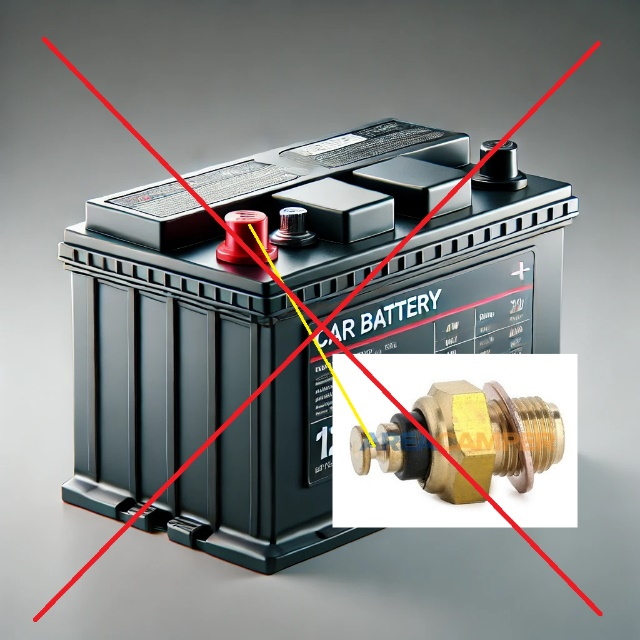
\includegraphics[width=\linewidth]{digifiz_manual/image002.jpg}
        \caption{Warning supplied with the sensor harness against external voltage.}
    \end{subfigure}
    \caption{Safety placards shipped with the wiring kit.}
\end{figure}

\chapternotnumbered{Introduction} \label{ch:Introduction}

This user manual consolidates the build notes, service procedures, and release checklists gathered while shipping Digifiz Replica dashboards across two hardware generations.
The \TeXtured{} template powering the document was iterated on for years to balance production-ready typography with a modular source layout that stays maintainable as the manual grows.

Refining the template for technical documentation meant embracing theorem-like and remark-like environments for tightly connected references, and investing into automation so that metadata, figures, and indexes stay synchronized between revisions.
Improved understanding of the coding backbone behind \LaTeX{} and its package ecosystem enabled me to customize it even further to my liking, and add even more \enquote{bells and whistles}.

\begin{remark}[Template Purpose]
    While this project focuses on the Digifiz Replica user manual, \TeXtured{} can be used for other long-form technical documents as well.
\end{remark}

To make it user-friendly, I have restructured the preamble into several files, each of which is responsible for a specific aspect of the document.
This way, the user can (and is encouraged to) easily find the relevant part of the code and modify it.

Numerous comments and explanations are provided throughout the code to further aid the user in understanding the template without always having to consult the documentation of packages (which is recommended for more advanced changes).

\begin{remark}[How to Setup]
    To set up \TeXtured{} template for your document, you can use the \texttt{Overleaf} template or clone the repository on \textsf{GitHub} \autocite{TeXtured}.
    Then, you can start modifying the files to suit your needs.

    Also make sure to check the \texttt{README.md} file for more detailed instructions, particularly on various software dependencies.
    If you encounter any issues, please see \href{https://github.com/jdujava/TeXtured/issues/2}{\texttt{jdujava/TeXtured \#2}} and \href{https://github.com/jdujava/TeXtured/issues/5}{\texttt{jdujava/TeXtured \#5}}.
\end{remark}

\chapter{Description and operation of the product}\label{ch:description}

\section{Purpose}
The \ReplicaGenOne{} and \ReplicaNextLong{} dashboards replace the original Volkswagen instrument clusters while extending their functionality. They provide digital indications for speed, engine speed, coolant temperature, fuel level, and auxiliary MFA calculations, and they support both cable and electronic speed sensors. \ReplicaGenOneShort{} units integrate a Bluetooth controller, while \ReplicaNextShort{} adds Wi-Fi-based configuration modules and optional expansion units.

\section{Model identification}
Every dashboard is marked with a four-letter code that describes the drivetrain, assembly type, speed sensor interface, and wiring generation. Optional digits indicate the supported tachometer scale, and an additional three-letter suffix reports export measurement units.

\subsection{Four-letter designation}
\begin{description}
    \item[Position~1] \textbf{G} for petrol engines or \textbf{D} for diesel engines.
    \item[Position~2] \textbf{A} for factory-assembled units or \textbf{M} for self-assembly kits.
    \item[Position~3] \textbf{C} for a mechanical cable speed sensor or \textbf{R} for an electronic speed sensor.
    \item[Position~4] \textbf{T} for the pre-facelift (CE~1) harness or \textbf{S} for the facelift (CE~2) harness.
\end{description}
A trailing digit denotes the maximum displayed engine speed in thousands of RPM (for example, “8” on a GACT8 cluster equals an 8000~RPM scale).

\subsection{Measurement suffix}
Export variants may add a three-letter suffix formed from the set \texttt{MGFK}:
\begin{description}
    \item[M] miles per hour,
    \item[G] gallons,
    \item[F] Fahrenheit,
    \item[K] Kelvin.
\end{description}
For example, a \texttt{GART8-MGF} dashboard is a petrol, factory-assembled, electronic-sensor, CE~2 unit with an 8000~RPM tachometer and imperial measurement units.

\section{Model range}
{\scriptsize
\begin{tblr}{
    colspec={Q[l,2.2cm] X[l]},
    hlines
}
\textbf{Model} & \textbf{Description} \\
GACT & Petrol, fully assembled, cable speed sensor, two connectors, 7000~RPM scale. \\
GART & Petrol, fully assembled, remote electronic speed sensor, two connectors, 7000~RPM scale. \\
GAC & Petrol, fully assembled, cable speed sensor, single connector, 7000~RPM scale. \\
GARS & Petrol, fully assembled, remote electronic speed sensor, single connector, 7000~RPM scale. \\
GACT8 & Petrol, fully assembled, cable speed sensor, two connectors, 8000~RPM scale. \\
GART8 & Petrol, fully assembled, remote electronic speed sensor, two connectors, 8000~RPM scale. \\
GACS8 & Petrol, fully assembled, cable speed sensor, single connector, 8000~RPM scale. \\
GARS8 & Petrol, fully assembled, remote electronic speed sensor, single connector, 8000~RPM scale. \\
DACT & Diesel, fully assembled, cable speed sensor, two connectors, 6000~RPM scale. \\
DART & Diesel, fully assembled, remote electronic speed sensor, two connectors, 6000~RPM scale. \\
DACS & Diesel, fully assembled, cable speed sensor, single connector, 6000~RPM scale. \\
DARS & Diesel, fully assembled, remote electronic speed sensor, single connector, 6000~RPM scale. \\
MT & Self-assembly kit with two connectors. \\
M.S. & Self-assembly kit with a single connector. \\
NEXT-GART & \ReplicaNextLong{}, 8000~RPM scale, two connectors, electronic speed sensor. \\
NEXT-GARS & \ReplicaNextLong{}, 8000~RPM scale, single connector, electronic speed sensor. \\
NEXT-MT & \ReplicaNextLong{} self-assembly kit with two connectors. \\
NEXT-MS & \ReplicaNextLong{} self-assembly kit with a single connector. \\
\end{tblr}}

\section{Connector pin-outs}
\subsection{Clusters with two connectors}
\begin{figure}[htbp]
    \centering
    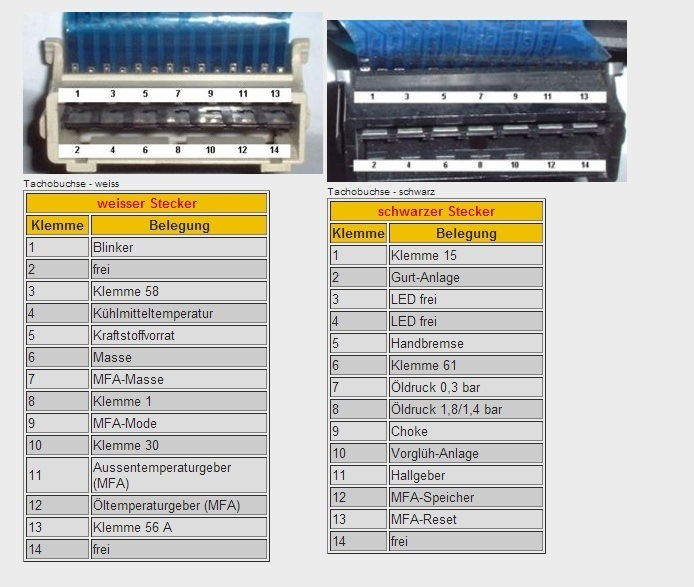
\includegraphics[width=0.72\textwidth]{digifiz_manual/image008.jpg}
    \caption{Connector layout for dual-connector \ReplicaGenOne{} dashboards.}
\end{figure}

\noindent\textbf{White connector}

{\scriptsize
\begin{tblr}{
    colspec={Q[l,1.4cm] X[l]},
    hlines
}
\textbf{Pin} & \textbf{Assignment} \\
1 & Blinker output, tied to ground for the indicator lamp. \\
2 & Frei --- not connected. \\
3 & Terminal~58, positive supply for the panel backlight. \\
4 & Resistive coolant temperature sensor input. \\
5 & Resistive fuel level sensor input. \\
6 & Ground return. \\
7 & Additional ground return. \\
8 & Terminal~1 engine-speed signal (coil, distributor, or other waveform up to 12~V with possible 300~V spikes). \\
9 & MFA mode line used to change MFA functions. \\
10 & UNR permanent positive supply (unused on \ReplicaGenOneShort{}, main supply on \ReplicaNextShort{}). \\
11 & MFA temperature “+” lead for the ambient sensor (\ReplicaNextShort{}). \\
12 & MFA oil temperature sensor lead (\ReplicaNextShort{} only). \\
13 & KL~56a high-beam indicator input (+12~V active). \\
\end{tblr}}

\noindent\textbf{Black connector}

{\scriptsize
\begin{tblr}{
    colspec={Q[l,1.4cm] X[l]},
    hlines
}
\textbf{Pin} & \textbf{Assignment} \\
1 & Terminal~15 switched +12~V from the ignition switch. \\
2--4 & Not connected. \\
5 & Handbrake indicator input (active low). \\
6 & KL~61 generator warning lamp drive with 120~\ensuremath{\Omega} excitation resistor. \\
7 & Oil pressure switch, 0.3~bar. \\
8 & Oil pressure switch, 1.8~bar. \\
9 & Not used. \\
10 & Glow-plug indicator input (+12~V active, diesel only). \\
11 & Hall sensor input for optional speed sensors. \\
12 & MFA block selection line. \\
13 & MFA reset line. \\
\end{tblr}}

\subsection{Clusters with a single connector}
Single-connector dashboards use the mapping shown in \autoref{fig:single-connector}. The harness replicates the same signals found on the dual-connector variants but consolidates them into a single plug.

\begin{figure}[htbp]
    \centering
    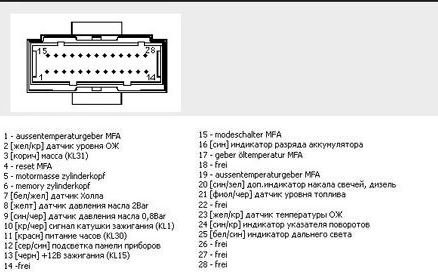
\includegraphics[width=0.65\textwidth]{digifiz_manual/image009.png}
    \caption{Single-connector layout used on compact Replica dashboards.}
    \label{fig:single-connector}
\end{figure}

\subsection{Scirocco prospective harness}
The prospective Scirocco harness uses two plugs:
\begin{description}
    \item[5-pin plug]
        1.~D3, 2.~D2, 3.~D1, 4.~SA, 5.~SPERRE.
    \item[14-pin plug]
        1.~KL~58, 2.~MASS, 3.~TANK, 4.~TEMP, 5.~KL~1, 6.~UHR, 7.~FERNL, 8.~(reserved), 9.~OEL~1.8, 10.~CAT~VORGL(-), 11.~OEL~0.3, 12.~KL~61, 13.~KL~49a (blinker), 14.~KL~15.
\end{description}

\subsection{Mk1 connector mapping}
Volkswagen Mk1 vehicles use the following assignments:
\begin{enumerate}
    \item Illumination and low-beam supply.
    \item MASSE~31 ground reference.
    \item TANK fuel-level sender.
    \item TEMP coolant temperature sender.
    \item KL~1 tachometer signal.
    \item UHR permanent +12~V.
    \item KL~56 high-beam signal.
    \item OIL (HIGH) 1.8~bar pressure switch.
    \item OIL (LOW) 0.3~bar pressure switch.
    \item Diesel glow indicator.
    \item CHOKE input (unused).
    \item KL~61 generator lamp.
    \item Blinker input (combined left/right).
    \item KL~15 ignition supply.
\end{enumerate}
\begin{figure}[htbp]
    \centering
    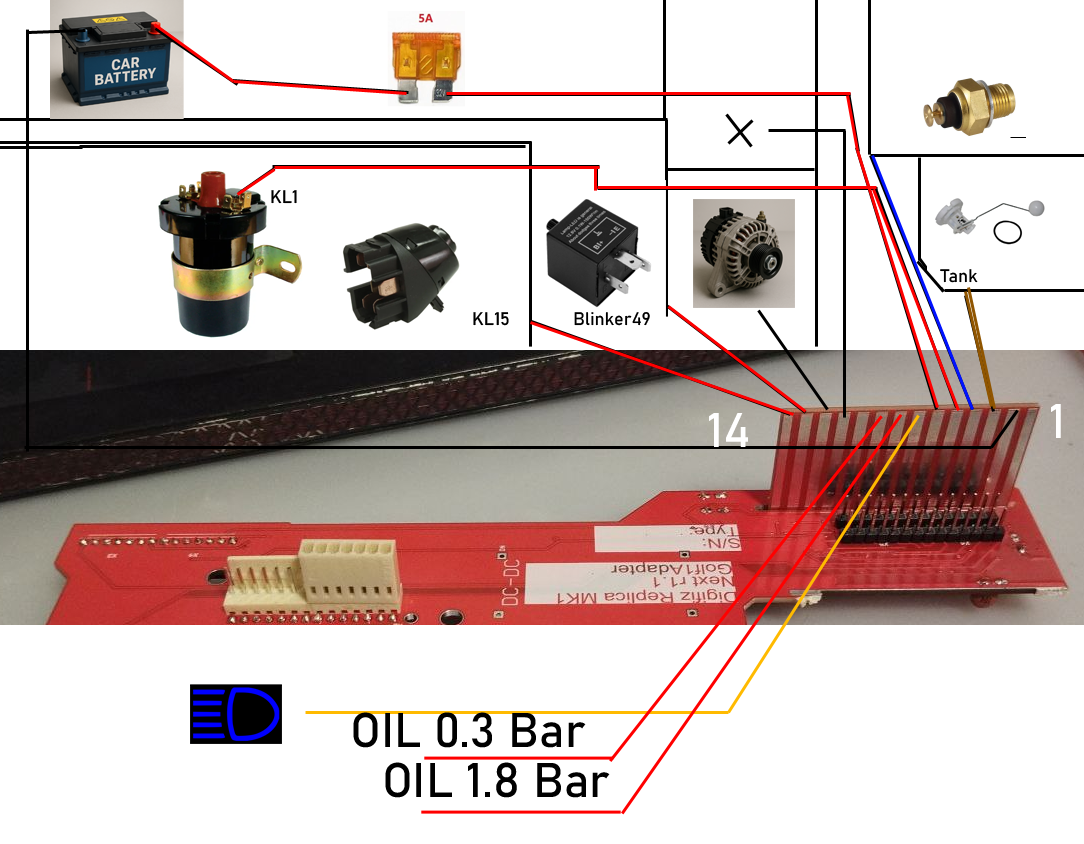
\includegraphics[width=0.75\textwidth]{digifiz_manual/image010.png}
    \caption{Harness connection diagram for Mk1 installations.}
\end{figure}

\subsection{Printed-circuit-board service connector}
The third connector on the circuit board mirrors the dashboard connectors, with pins numbered right-to-left on \ReplicaGenOneShort{} and \ReplicaNextShort{} units. It provides a service interface with the assignments listed in \autoref{tab:service-connector}.

\begin{table}[htbp]
    \centering
    \caption{Service connector pin assignments.}
    \label{tab:service-connector}
    {\scriptsize
    \begin{tblr}{
        colspec={Q[l,1.9cm] X[l]},
        hlines,
    }
        \textbf{Position} & \textbf{Assignment} \\
        1 & Indicator output. \\
        2 & Speed sensor input (SPM\_M). \\
        3 & Vehicle ground. \\
        4 & Indicator output. \\
        5 & Left blinker optocoupler input. \\
        6 & Right blinker optocoupler input. \\
        7 & Ignition +12~V. \\
        8 & Diesel-specific input. \\
        9 & Indicator input (positive). \\
        10 & Alternative RPM input (unused, \ReplicaNextShort{} only). \\
        11 & \ReplicaGenOneShort{}: indicator output (normally disconnected); \ReplicaNextShort{}: brake input (active low). \\
        12 & Reserved. \\
        13 & Check-engine input. \\
        14 & No contact. \\
    \end{tblr}}
\end{table}

\section{Embedded software and completeness}
The dashboard firmware is published at \url{https://github.com/Sgw32/DigifizReplica}. Two delivery sets are available:
\begin{itemize}
    \item \textbf{\ReplicaGenOne{}:} dashboard assembly, ambient and oil temperature harness, USBasp programmer, and (for remote sensors) a speed sensor harness.
    \item \textbf{\ReplicaNextLong{}:} dashboard assembly and an electronic speed sensor harness.
\end{itemize}

\chapter{Operating Principle} \label{ch:operating-principle}

Digifiz Replica dashboards reuse the original Volkswagen enclosure, the factory CE~1 or CE~2 connectors, and either the mechanical speedometer cable or an electronic speed sensor.
Replica main boards are based on a fiberglass PCB populated with discrete components controlled by an ATmega~2560 microcontroller and MAX~7219 indicator drivers.

Digifiz Replica Next builds on an ESP32-S3 system-on-chip and introduces a newly manufactured SLA-printed enclosure, a redesigned front panel and cover, and a connector adapter board.
The Next-generation display is illuminated by WS2812 addressable LEDs mounted behind the front frame, and the accompanying harness includes the electronic speed sensor by default.

Both generations share the same display layout and MFA pages, ensuring that installation procedures and day-to-day operation remain familiar between hardware revisions.

\chapter{Technical specifications}\label{ch:technical-specs}

The Digifiz Replica dashboard consumes no standby current when powered down. Digifiz Replica Next draws approximately 13~mA from the +12~V supply while the ignition is off, which should be considered when the vehicle is stored for extended periods. Both generations operate reliably from the vehicle electrical system between 9~V and 16~V~DC.

\section{Measurement capabilities}
\begin{itemize}
    \item \textbf{Vehicle speed:} measured through the factory cable or electronic speed sensor. The systematic error is 10~km/h, the relative error is 3~km/h, and the indication saturates at 999~km/h (or mph for imperial units).
    \item \textbf{Engine speed:} derived from the ignition signal via an optocoupler stage with a 430~nF/1.2~k\ensuremath{\Omega} RC network and a diode limiter. The absolute and relative errors are within 200~rpm.
    \item \textbf{Fuel level:} read from the resistive tank sender with an uncertainty of approximately 10~litres.
    \item \textbf{Coolant temperature:} indicated qualitatively using the standard thermistor connected through the vehicle harness; quantitative values are not displayed.
    \item \textbf{Timekeeping:} maintained to within one minute.
    \item \textbf{Indicator lamps:} direction indicators, high beam, oil pressure warnings, generator status, handbrake, rear window heating or diesel glow-plug, and front and rear fog lights.
\end{itemize}

\chapter{Operating conditions and safety precautions}\label{ch:safety}

\section{Environmental limits}
\begin{itemize}
    \item The instrument panel operates between \(-40\,^{\circ}\mathrm{C}\) and \(+70\,^{\circ}\mathrm{C}\) at relative humidity up to 95~\%.
    \item The dashboard may remain installed inside the vehicle throughout the year, including when the car is parked for extended periods.
\end{itemize}

\section{Safety precautions}
\begin{enumerate}
    \item The Digifiz dashboard is a do-it-yourself device assembled and integrated by enthusiasts. Observe general electrical safety practices while working with it.
    \item The product is intended for the personal projects of vehicle owners.
    \item The readings are not certified or metrologically verified, although they correspond to the declared specifications at the time of release.
    \item Use the dashboard only when you accept responsibility for the installation and for road safety.
    \item If the displayed data cannot be trusted, verify it with the vehicle's standard gauges or external measuring instruments.
    \item Do not use the instrument panel outputs for automatic vehicle control systems.
    \item The authors accept no liability for consequences arising from the installation or use of the dashboard, including traffic fines or accidents. Malfunctions reported within the warranty period (one year for installations performed jointly with the authors and two weeks for independent installations) will be repaired.
    \item The functional capabilities listed in \Cref{ch:technical-specs} are guaranteed for one year during supervised installation and for two weeks after independent installation.
\end{enumerate}

\chapter{Preparation for work and work order}\label{ch:preparation}

\section{Preparing the vehicle}
Follow the sequence below when replacing the factory cluster with a Digifiz dashboard:
\begin{enumerate}
    \item Remove the plastic trim covering the pedals and the lower dashboard to expose the original instrument panel.
    \item Disconnect the vehicle battery.
    \item Unplug the wiring harness from the factory instrument panel.
    \item Detach the mechanical speedometer cable, if present.
    \item Unscrew the panel from its brackets and carefully remove it from the vehicle.
    \item Route the supplied temperature and speed sensor harnesses as required.
    \item Install the Digifiz dashboard into the bracket grooves and secure it with screws.
    \item For \ReplicaNextLong{}, install the Volkswagen MFA sensors (or equivalents) and route their leads to the CE~1/CE~2 connectors.
    \item On \texttt{GACS}/\texttt{GARS}/\texttt{DARS}/\texttt{DACS} models, connect the labelled \texttt{MFA\_MODE}, \texttt{MFA\_RESET}, \texttt{MFA\_BLOCK}, and handbrake wires manually if the vehicle harness lacks these contacts. The second-generation \ReplicaNextShort{} connects these signals internally by default.
    \item Plug the harnesses into the dashboard.
    \item Fit the electronic speed sensor or reconnect the mechanical cable.
    \item Reinstall the dashboard trim and pedal cover in the reverse order.
\end{enumerate}

\section{Operating the dashboard}
\begin{itemize}
    \item The dashboard powers up automatically with the ignition. The sidelights switch controls the backlight.
    \item At start-up the entire speed scale illuminates while internal diagnostics stabilise the RPM model; the display then settles on the current idle speed.
    \item Once the vehicle begins to move, the system reports the parameters listed in \Cref{ch:technical-specs}.
\end{itemize}

\subsection{MFA functions}
Six MFA pages are available:
\begin{enumerate}
    \item Daily operating time.
    \item Trip distance.
    \item Fuel consumption (not implemented on the first Replica revision).
    \item Average speed (displayed as the value multiplied by ten).
    \item Engine oil temperature (external harness required).
    \item Ambient temperature (external harness required).
\end{enumerate}
On \ReplicaGenOneShort{} dashboards a capacitive touch point behind the VW badge cycles the pages; \ReplicaNextShort{} uses an external steering-column switch. Touch durations behave as follows:
\begin{itemize}
    \item Short press (\(<1\)~s): cycle to the next MFA function.
    \item Medium press (1--3~s when no steering-column switch is fitted): switch between MFA memory blocks; the change is indicated on screen.
    \item Long press (3--7~s): reset the active MFA function (affecting consumption, trip distance, elapsed time, and average speed).
\end{itemize}

\subsection{Backlight and indicator layout}
The \ReplicaGenOneShort{} dashboard offers a manual brightness trim above the parking-light switch; \ReplicaNextShort{} relies on automatic brightness driven by a photodiode. Manual overrides can be configured through the maintenance interfaces described in \Cref{ch:replica-setup,ch:replica-next-setup}.

The layout of the horizontal indicator block and the on-screen legend are shown in \autoref{fig:indicator-layout}.

\begin{figure}[htbp]
    \centering
    \begin{subfigure}{0.48\textwidth}
        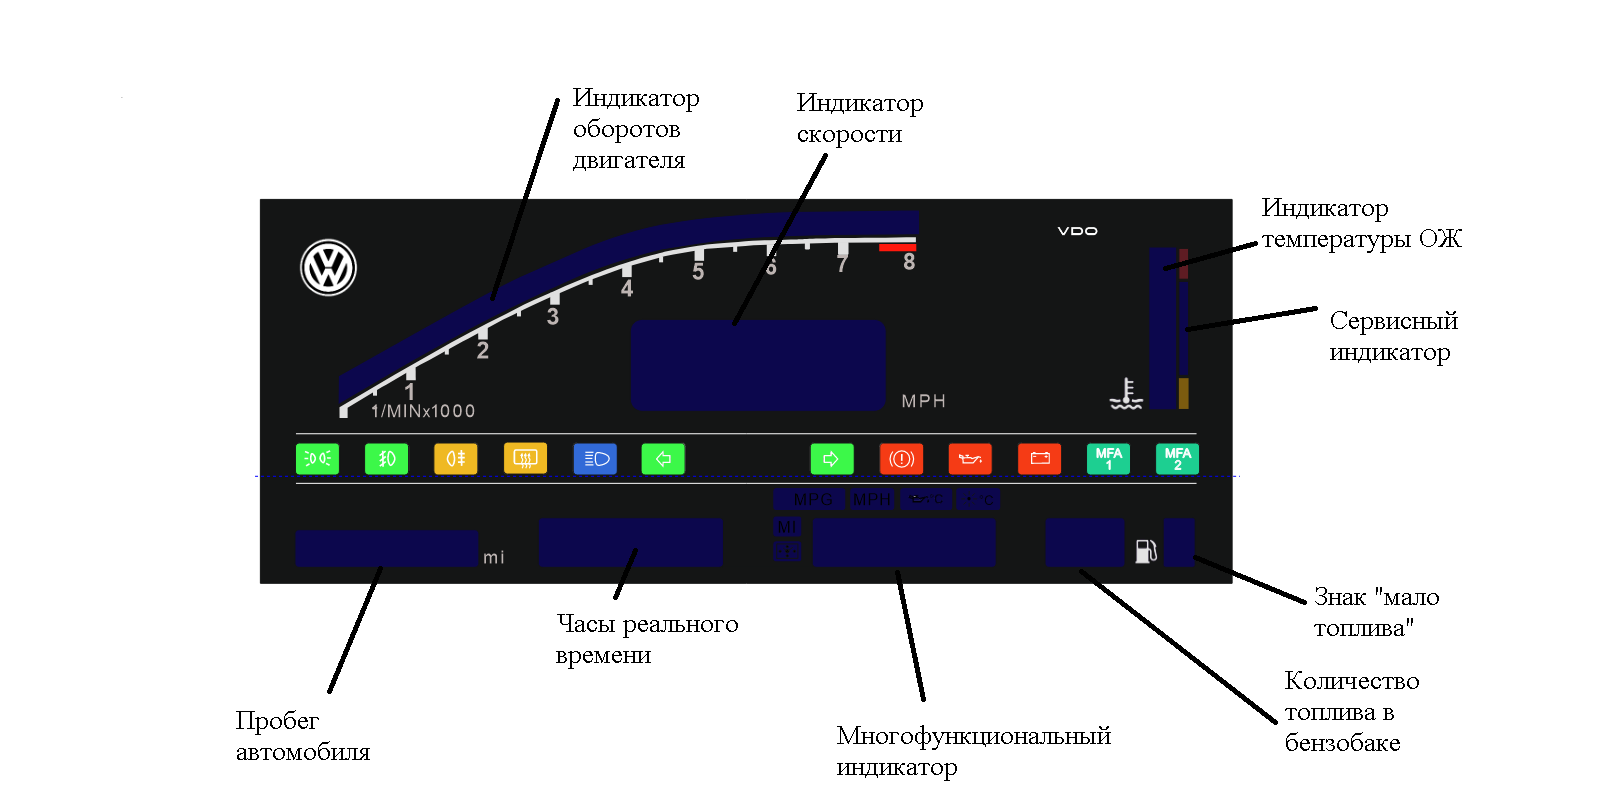
\includegraphics[width=\linewidth]{digifiz_manual/image017.png}
        \caption{Indicator layout displayed during the power-on self-test.}
    \end{subfigure}\hfill
    \begin{subfigure}{0.48\textwidth}
        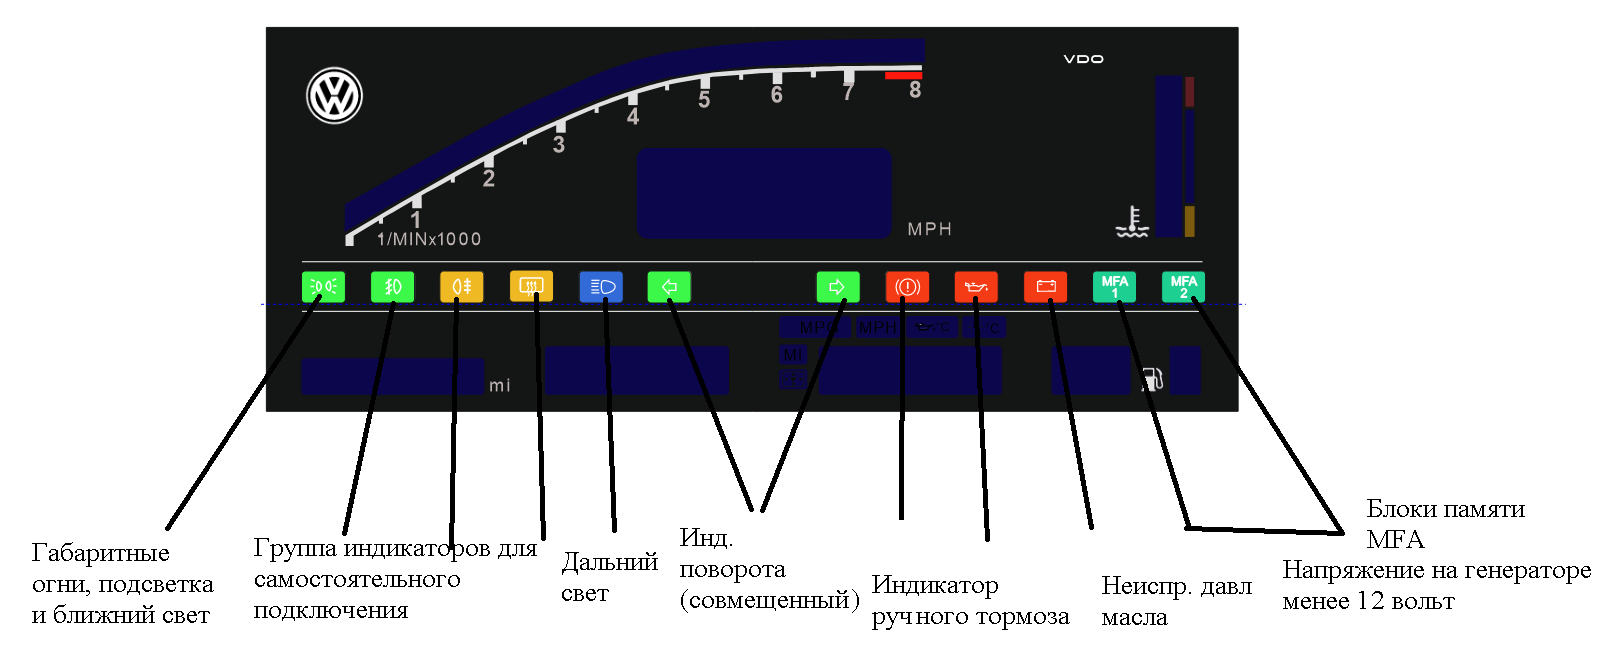
\includegraphics[width=\linewidth]{digifiz_manual/image018.png}
        \caption{Legend for the horizontal indicator group.}
    \end{subfigure}
    \caption{Instrument panel indication scheme.}
    \label{fig:indicator-layout}
\end{figure}

\subsection{Configuration interfaces}
\begin{itemize}
    \item Classic \ReplicaGenOne{} units include a Bluetooth 2.0 (or BLE-compatible) module. Install the \emph{Serial Bluetooth Terminal} application from Google Play, pair with the dashboard, and issue commands directly from the terminal view. Apple iOS devices cannot connect to this module.
    \item \ReplicaNextShort{} exposes an embedded Wi-Fi access point and configuration portal described in \Cref{ch:replica-next-setup}. Disable mobile data while connecting to ensure the captive portal loads correctly.
\end{itemize}
Both generations can also be powered and configured on the bench using the USBasp programming interface.

\chapter{Setting up and maintaining Digifiz Replica Next}\label{ch:replica-next-setup}

This section applies to the Digifiz Replica Next dashboard shown in \autoref{fig:next-hardware}.

\begin{figure}[htbp]
    \centering
    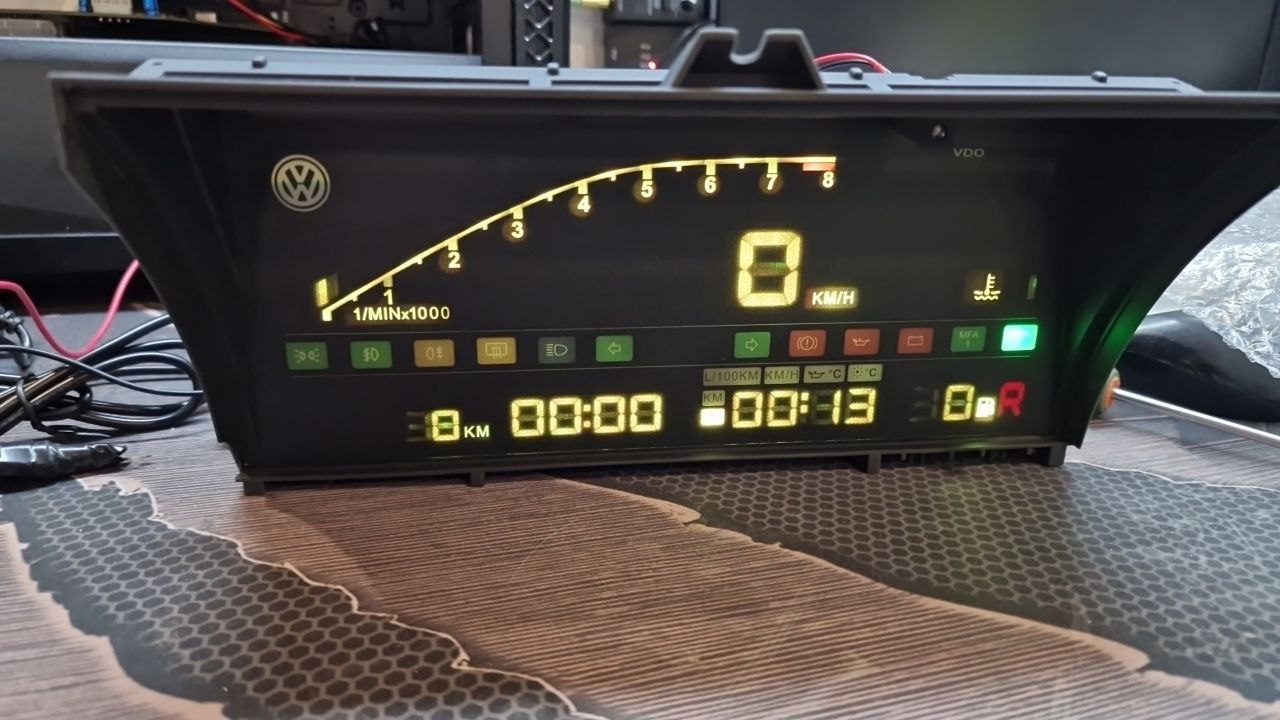
\includegraphics[width=0.6\textwidth]{digifiz_manual/image019.png}
    \caption{Digifiz Replica Next dashboard assembly.}
    \label{fig:next-hardware}
\end{figure}

\section{Panel handling}
\begin{itemize}
    \item The UV-printed polycarbonate faceplate must be protected from scratches and foreign objects. Significant damage requires replacement parts and is not treated as a warranty case.
    \item The real-time clock is configured via the Wi-Fi control panel. It resets whenever the permanent supply is disconnected.
\end{itemize}

\section{Wi-Fi control portal}
Configuration, data collection, and firmware management are performed through the embedded web application.
\begin{itemize}
    \item Connect to the dashboard's Wi-Fi access point. Disable mobile data and join \texttt{Digifiz\_AP} (password \texttt{87654321}); some revisions advertise \texttt{PHOL-LABS2} with the same password.
    \item The default IP address is \texttt{192.168.4.1}. If the dashboard is configured to join another network, scan the subnet for an address ending in \texttt{.32} using an IP tools application.
    \item The portal contains three tabs: \emph{WiFi}, \emph{Control}, and \emph{About} (\autoref{fig:next-control-tabs}). The Wi-Fi tab configures network settings and handles firmware uploads; the Control tab adjusts dashboard parameters; the About tab lists author information.
\end{itemize}

\begin{figure}[htbp]
    \centering
    \begin{subfigure}{0.48\textwidth}
        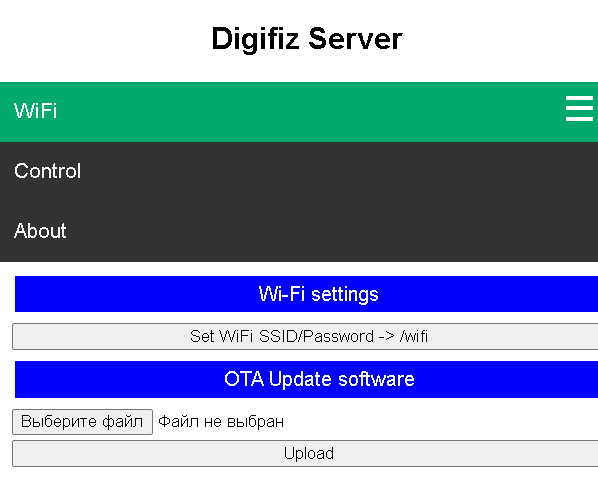
\includegraphics[width=\linewidth]{digifiz_manual/image020.png}
        \caption{Control tab overview.}
    \end{subfigure}\hfill
    \begin{subfigure}{0.48\textwidth}
        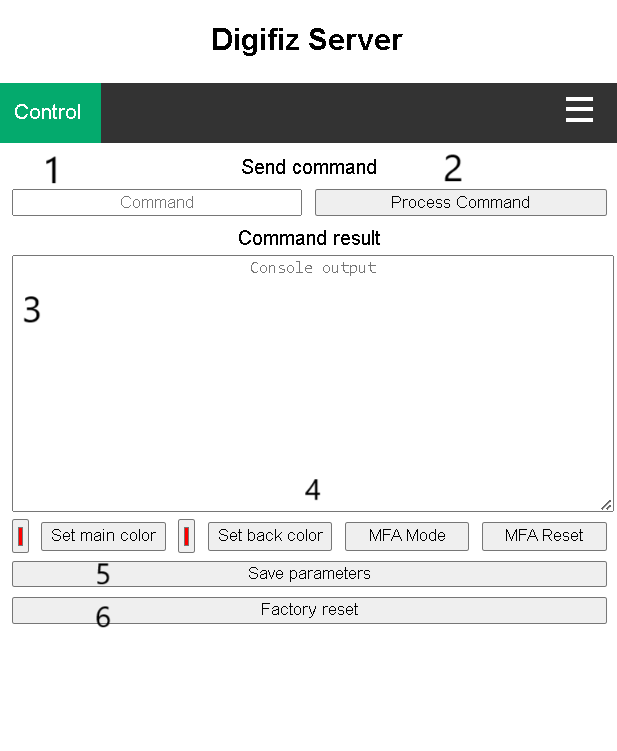
\includegraphics[width=\linewidth]{digifiz_manual/image021.png}
        \caption{Numbered controls and command entry fields.}
    \end{subfigure}
    \caption{Replica Next Wi-Fi control interface.}
    \label{fig:next-control-tabs}
\end{figure}

\section{Command entry}
The \emph{Control} tab provides a command input line (1), a \emph{Process} button (2), a result window (3), quick controls (4), a \emph{Save} button (5), and a \emph{Reset} button (6). Enter commands as space-separated pairs \verb|<number> <value>| using integers only; punctuation and quotation marks are not required. \autoref{fig:next-command-example} illustrates the interface while toggling automatic brightness.

\begin{figure}[htbp]
    \centering
    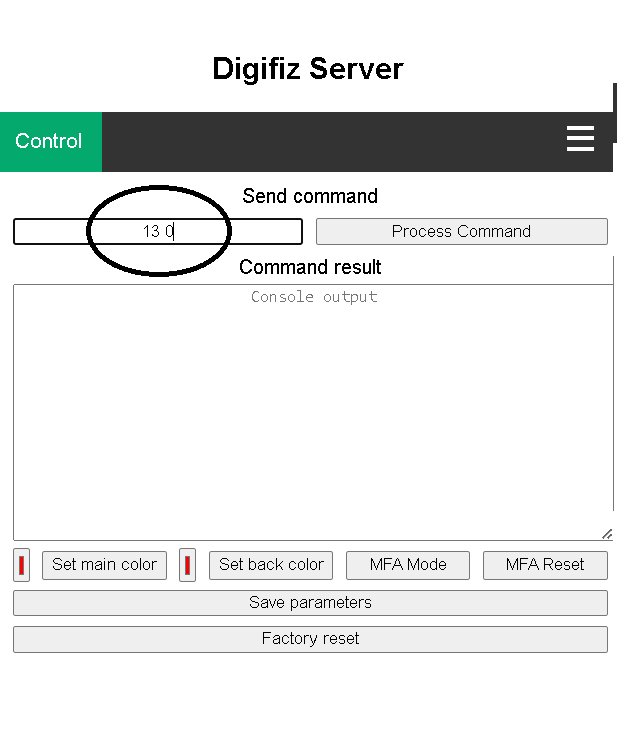
\includegraphics[width=0.55\textwidth]{digifiz_manual/image022.png}
    \caption{Example command sequence disabling automatic brightness.}
    \label{fig:next-command-example}
\end{figure}

\section{Command reference}
\begin{table}[htbp]
    \centering
    \caption{Primary Replica Next configuration commands.}
    \label{tbl:next-commands}
    \begin{tblr}{
        colspec = {>{\ttfamily}Q[c,0.12\linewidth] Q[l] Q[l]},
        row{1} = {font=\bfseries},
        rowsep = 2pt,
    }
        \toprule
        Command & Name & Description \\
        \midrule
        22 (or 0) & PARAMETER\_RPMCOEFFICIENT & Engine RPM calibration factor (100--10000). \\
        1  & PARAMETER\_SPEEDCOEFFICIENT & Speed calibration factor (10--255). \\
        2  & PARAMETER\_COOLANTTHERMISTORB & Coolant thermistor beta coefficient (2000--5000). \\
        3  & PARAMETER\_OILTHERMISTORB & Oil thermistor beta coefficient (2000--5000). \\
        4  & PARAMETER\_AIRTHERMISTORB & Ambient thermistor beta coefficient (2000--5000). \\
        5  & PARAMETER\_TANKMINRESISTANCE & Minimum fuel sender resistance (0--1000~\ohm). \\
        6  & PARAMETER\_TANKMAXRESISTANCE & Maximum fuel sender resistance (100--1000~\ohm). \\
        7  & PARAMETER\_TAU\_COOLANT & Coolant temperature filter constant (1--50, higher is more responsive). \\
        8  & PARAMETER\_TAU\_OIL & Oil temperature filter constant (1--50). \\
        9  & PARAMETER\_TAU\_AIR & Ambient temperature filter constant (1--50). \\
        10 & PARAMETER\_TAU\_TANK & Fuel level filter constant (1--50). \\
        11 & PARAMETER\_MILEAGE & Total odometer value (0--999999). \\
        12 & PARAMETER\_DAILY\_MILEAGE & Trip odometer (0--9999). \\
        13 & PARAMETER\_AUTO\_BRIGHTNESS & Automatic brightness enable (1=on, 0=off). \\
        14 & PARAMETER\_BRIGHTNESS\_LEVEL & Manual brightness level (0--60\%; values above 60 reduce LED life). \\
        15 & PARAMETER\_TANK\_CAPACITY & Fuel tank capacity in litres (0--99; 55~L typical for Golf~2). \\
        16 & PARAMETER\_MFA\_STATE & Active MFA mode (normally controlled via hardware input). \\
        17 & PARAMETER\_BUZZER\_OFF & Disable buzzer (1 disables, 0 enables; Replica Next lacks a buzzer). \\
        18 & PARAMETER\_MAX\_RPM & Tachometer scaling (typical 8000, range 4000--16000). \\
        19 & PARAMETER\_NORMAL\_RESISTANCE\_COOLANT & Coolant sensor resistance at 25\,^{\circ}C (1000--10000~\ohm). \\
        20 & PARAMETER\_NORMAL\_RESISTANCE\_OIL & Oil sensor resistance at 25\,^{\circ}C (1000--10000~\ohm). \\
        21 & PARAMETER\_NORMAL\_RESISTANCE\_AMB & Ambient sensor resistance at 25\,^{\circ}C (1000--10000~\ohm). \\
        23 & PARAMETER\_DOT\_OFF & Clock colon behaviour (0=blink, 1=solid). \\
        24 & PARAMETER\_BACKLIGHT\_ON & Enable backlight on low beam (not used on Replica Next). \\
        25 & PARAMETER\_M\_D\_FILTER & Median filter constant (legacy, normally unused). \\
        26 & PARAMETER\_COOLANT\_MAX\_R & Coolant sensor threshold for full-scale indication (100--150~\,^{\circ}C). \\
        27 & PARAMETER\_COOLANT\_MIN\_R & Coolant sensor threshold for ``1~bar'' indication (0--80~\,^{\circ}C). \\
        31 & PARAMETER\_MAINCOLOR\_R & Red component of the UI colour (0--255). \\
        32 & PARAMETER\_MAINCOLOR\_G & Green component of the UI colour (0--255). \\
        33 & PARAMETER\_MAINCOLOR\_B & Blue component of the UI colour (0--255). \\
        37 & PARAMETER\_RPM\_FILTER & RPM filter aggressiveness (10--200, higher reacts faster). \\
        128 & PARAMETER\_READ\_ADDITION & Add 128 to read the current value of any command. \\
        255 & PARAMETER\_SET\_HOUR & Set clock hours (24-hour format). \\
        254 & PARAMETER\_SET\_MINUTE & Set clock minutes. \\
        253 & PARAMETER\_RESET\_DAILY\_MILEAGE & Reset the trip odometer. \\
        252 & PARAMETER\_RESET\_DIGITAL & Factory reset of stored parameters. \\
        \bottomrule
    \end{tblr}
\end{table}

\section{Default values}
\begin{table}[htbp]
    \centering
    \caption{Replica Next default settings.}
    \label{tbl:next-defaults}
    \begin{tblr}{
        colspec = {>{\ttfamily}Q[c,0.18\linewidth] Q[c,0.18\linewidth] Q[l]},
        row{1} = {font=\bfseries},
        rowsep = 2pt,
    }
        \toprule
        Parameter & Default & Notes \\
        \midrule
        PARAMETER\_RPMCOEFFICIENT & 3000 & Typical for Audi tachometer inputs. \\
        PARAMETER\_SPEEDCOEFFICIENT & 100 & Calibrated for 100~km/h. \\
        PARAMETER\_COOLANTTHERMISTORB & 4000 &  \\
        PARAMETER\_OILTHERMISTORB & 4000 &  \\
        PARAMETER\_AIRTHERMISTORB & 3812 & 3600 for Generation~2 panels. \\
        PARAMETER\_TANKMINRESISTANCE & 35 & \ohm. \\
        PARAMETER\_TANKMAXRESISTANCE & 265 & \ohm. \\
        PARAMETER\_TAU\_COOLANT & 2 & Filter constant. \\
        PARAMETER\_TAU\_OIL & 2 & Filter constant. \\
        PARAMETER\_TAU\_AIR & 2 & Filter constant. \\
        PARAMETER\_TAU\_TANK & 2 & Filter constant. \\
        PARAMETER\_MILEAGE & Vehicle-specific & Retains stored odometer. \\
        PARAMETER\_DAILY\_MILEAGE & 0 &  \\
        PARAMETER\_AUTO\_BRIGHTNESS & 1 & Enabled. \\
        PARAMETER\_BRIGHTNESS\_LEVEL & 25 & Generation~2 default; Generation~1/1.5 use 7 or 13. \\
        PARAMETER\_TANK\_CAPACITY & 63 & Litres. \\
        PARAMETER\_MFA\_STATE & 0 & Default MFA page. \\
        PARAMETER\_BUZZER\_OFF & 1 & Buzzer disabled. \\
        PARAMETER\_MAX\_RPM & 8000 & Tachometer scale. \\
        PARAMETER\_NORMAL\_RESISTANCE\_COOLANT & 1000 & \ohm{} at 25\,^{\circ}C. \\
        PARAMETER\_NORMAL\_RESISTANCE\_OIL & 1000 & \ohm{} at 25\,^{\circ}C. \\
        PARAMETER\_NORMAL\_RESISTANCE\_AMB & 2991 & 500~\ohm{} for Generation~2 sensors. \\
        PARAMETER\_DOT\_OFF & 0 & Blinking clock colon. \\
        PARAMETER\_BACKLIGHT\_ON & 1 & Backlight enabled with low beam. \\
        PARAMETER\_M\_D\_FILTER & 65535 & Legacy median filter constant. \\
        PARAMETER\_COOLANT\_MAX\_R & 120 & \(^{\circ}\mathrm{C}\). \\
        PARAMETER\_COOLANT\_MIN\_R & 60 & \(^{\circ}\mathrm{C}\). \\
        PARAMETER\_MAINCOLOR\_R & 180 & Yellow-green default. \\
        PARAMETER\_MAINCOLOR\_G & 240 & Yellow-green default. \\
        PARAMETER\_MAINCOLOR\_B & 6 & Yellow-green default. \\
        PARAMETER\_RPM\_FILTER & 70 & Filter response. \\
        PARAMETER\_UPTIME & 0 & Runtime counter. \\
        \bottomrule
    \end{tblr}
\end{table}

\section{Reading parameters and examples}
To read a parameter, add 128 to the command number (for example, \verb|129 0| reports the speed coefficient). Typical commands include disabling automatic brightness (\verb|13 0|), enabling it again (\verb|13 1|), adjusting the speed coefficient (\verb|1 110| increases the displayed speed by roughly 5\%), and setting the odometer (\verb|11 123456|). Clock values are set with \verb|255 <hours>| followed by \verb|254 <minutes>|. Commands 31--33 set the RGB components of the user interface colour.

\section{Service commands}
Recent firmware revisions accept human-readable parameter names, for example \verb|PARAMETER_RPMCOEFFICIENT 3000|. The diagnostic command \verb|adc 0| prints raw ADC readings for sensor troubleshooting. Firmware updates add visual colour controls, so update regularly through the \emph{WiFi} tab to access the latest features.

\chapter{Typical situations for setting up the \ReplicaNextLong{}}\label{ch:replica-next-scenarios}

\begin{description}
    \item[Hotspot not visible] Move closer to the vehicle and ensure it is parked in an open area. Disable mobile data, forget stale Wi-Fi profiles, and reconnect to \texttt{Digifiz\_AP} (or \texttt{PHOL-LABS2}).
    \item[404 at \texttt{192.168.4.1}] Turn off mobile data on the phone or laptop and reload the page. Captive portal detection on Android/iOS often interferes until the cellular modem is disabled.
    \item[Firmware updates] Open the \emph{WiFi} tab and select the supplied \texttt{Digifiz.bin} file. The latest releases are published at the link below.
        \displayurl{https://github.com/Sgw32/DigifizReplica/releases}
        Click \emph{Upload}. The first attempt can fail; repeat the upload if necessary. Successful flashes redirect to a confirmation page. Record the odometer before updating and restore it afterwards with \verb|11 <mileage>|.
    \item[Commands ignored] Refresh the browser, return to the \emph{Control} tab, and resend the command. Ensure the \emph{Process} button is pressed after entering the value.
    \item[Speed reading incorrect] Connect via Wi-Fi, drive at an indicated \SI{100}{\kilo\metre\per\hour}, note the GPS speed, then issue \verb|1 <gps_value>| (for example, \verb|1 85|) to set \paramname{PARAMETER\_SPEEDCOEFFICIENT} to the verified value.
    \item[RPM reading incorrect] Adjust \paramname{PARAMETER\_RPMCOEFFICIENT}. Older firmware uses \verb|0 <value>|; current versions use \verb|22 <value>|. Example: \verb|22 1500| halves the reading relative to \verb|22 3000|.
    \item[Display too dim] Disable automatic brightness with \verb|13 0|, then raise the manual level (for example, \verb|14 50|). Experiment with values between 45 and 55; avoid levels above 60 to preserve LED life.
    \item[Setting the clock] Use the web terminal (or Serial Bluetooth Terminal on legacy builds) to send \verb|255 <hours>| followed by \verb|254 <minutes>|. Example: \verb|255 23| and \verb|254 55| sets 23:55.
    \item[Fuel readings stuck] Disconnect the battery and measure the resistance between the fuel sender pin and vehicle ground. Valid readings are typically \SIrange{30}{300}{\ohm}. Repair shorts below \SI{5}{\ohm} or open circuits before reconnecting. If the readings vary correctly but the gauge does not, record \verb|adc 0| results at several fuel levels and share them with PHOL-LABS Kft.
    \item[Fuel flow readings inaccurate] The optional flow sensor produces emulated data and is unreliable without an intake manifold pressure sensor. Treat the readings as experimental.
    \item[Coolant temperature out of range] Tune \paramname{PARAMETER\_COOLANT\_MIN\_R} and \paramname{PARAMETER\_COOLANT\_MAX\_R}. Example: \verb|27 30| lowers the ``1~bar'' threshold to \SI{30}{\celsius}.
    \item[Oil or ambient temperature missing] With the battery disconnected and the engine cold, measure the sensor resistance. Oil sensors should read about \SI{2}{\kilo\ohm} \ensuremath{\pm}\SI{0.3}{\kilo\ohm}, ambient sensors about \SI{10}{\kilo\ohm} \ensuremath{\pm}\SI{2}{\kilo\ohm}. Adjust \paramname{PARAMETER\_NORMAL\_RESISTANCE\_OIL} (command~20) or \paramname{PARAMETER\_NORMAL\_RESISTANCE\_AMB} (command~21); lower values decrease the indicated temperature, higher values increase it. Persistent issues should be diagnosed by collecting \verb|adc 0| output and contacting PHOL-LABS Kft.
    \item[Changing interface colour] Use commands 31--33 to set the RGB values. New firmware revisions include visual colour controls in the web interface, so update regularly.
\end{description}

\chapter{Setup and maintenance of the \ReplicaGenOne{}}\label{ch:replica-setup}

This chapter applies to the classic \ReplicaGenOne{} instrument panel shown in \autoref{fig:replica-classic}. If your dashboard matches the \ReplicaNextLong{} layout, refer to the previous chapter.

\begin{figure}[htbp]
    \centering
    \begin{subfigure}{0.46\textwidth}
        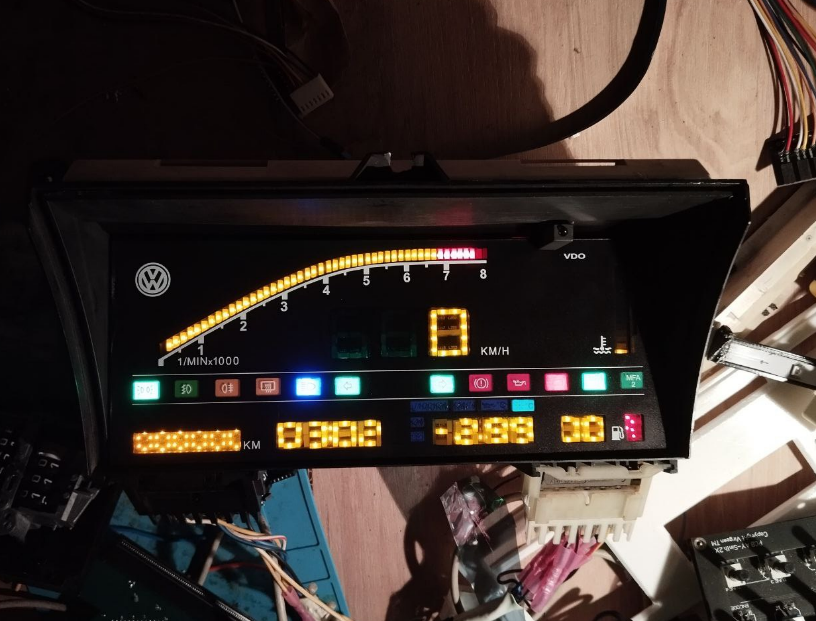
\includegraphics[width=\linewidth]{digifiz_manual/image046.png}
        \caption{Classic \ReplicaGenOne{} with square bezel.}
    \end{subfigure}\hfill
    \begin{subfigure}{0.46\textwidth}
        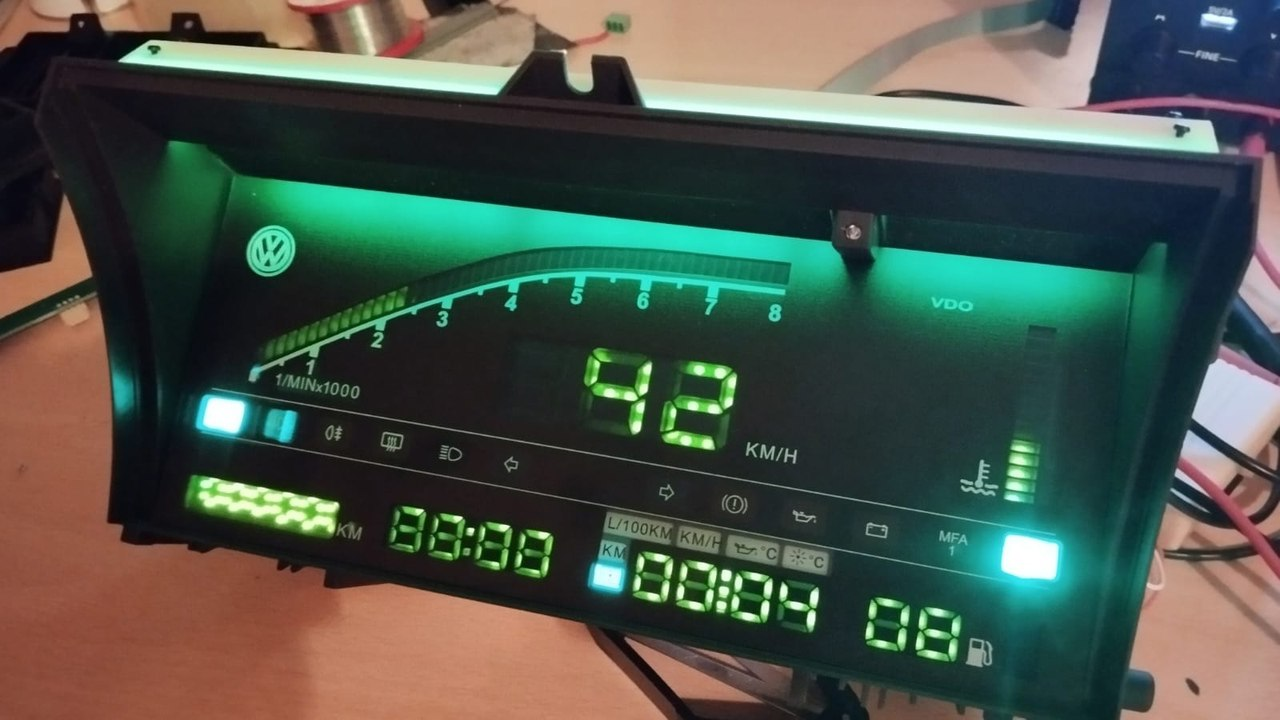
\includegraphics[width=\linewidth]{digifiz_manual/image047.png}
        \caption{Round-edge fascia used on later kits.}
    \end{subfigure}
    \caption{Appearance of the \ReplicaGenOne{} dashboard.}
    \label{fig:replica-classic}
\end{figure}

\section{Handling and screen care}
\begin{itemize}
    \item The plexiglass front with UV printing is easily marred. Avoid contact with sharp or abrasive objects.
    \item Surface damage is cosmetic and not covered by warranty. Request replacement parts from PHOL-LABS Kft if the screen pattern is deformed.
\end{itemize}

\section{Real-time clock battery}
The dashboard contains a DS3231 real-time clock with a CR2032 cell. The battery typically lasts about four years. When it is depleted the clock resets at every power-up. Remove the front and/or rear cover, keep the wiring harnesses connected, and replace the coin cell. Dispose of the spent battery according to local regulations.

\section{Firmware maintenance with USBasp}
Each kit ships with a USBasp programmer lead already connected inside the housing (\autoref{fig:usbasp-cable}). Install a suitable USBasp driver (for example from \url{https://myrobot.ru/downloads/driver-usbasp-v-2.0-usb-isp-windows-7-8-10-xp.php}) before flashing. The programmer powers the dashboard when it is connected to a computer, allowing bench checks.

\begin{figure}[htbp]
    \centering
    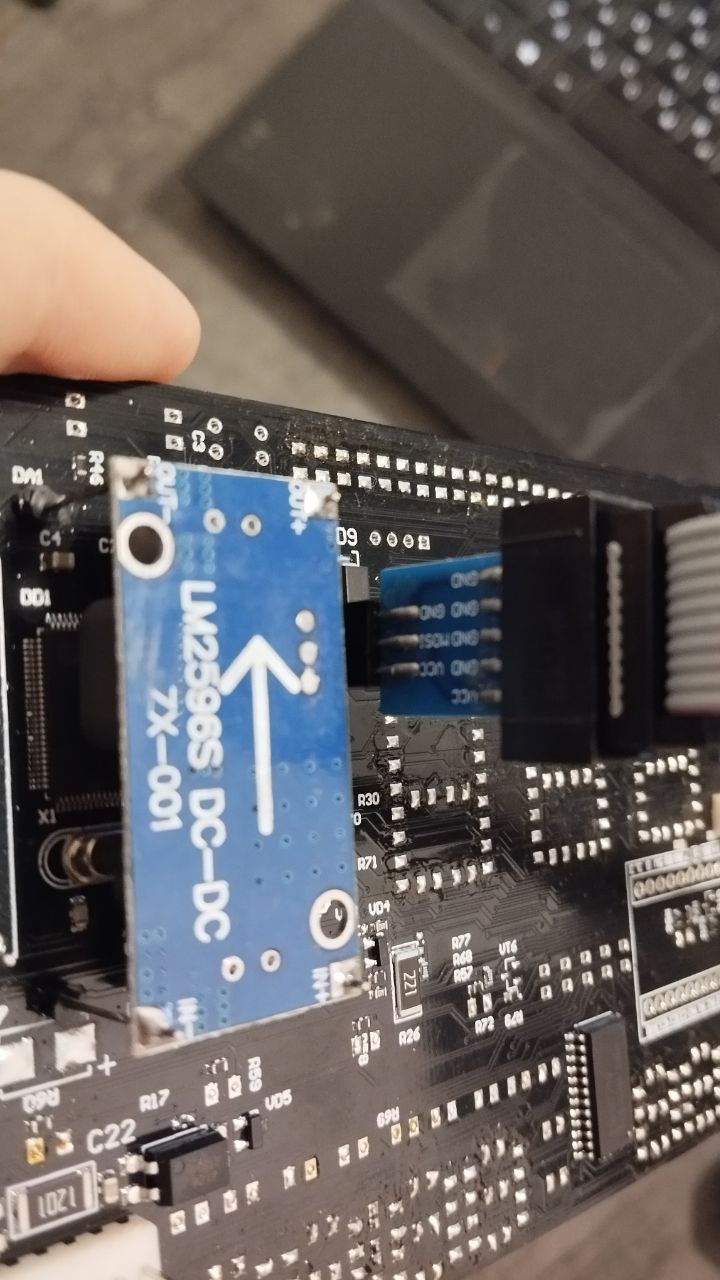
\includegraphics[width=0.32\textwidth]{digifiz_manual/image048.png}
    \caption{USBasp harness orientation inside the \ReplicaGenOne{}.}
    \label{fig:usbasp-cable}
\end{figure}

Flash firmware with \texttt{avrdude} using the command below (replace the firmware filename if required):

\begin{verbatim}
avrdude -c usbasp -p m2560 -e \
    -U lfuse:w:0xff:m -U hfuse:w:0x99:m -U efuse:w:0xff:m \
    -U flash:w:Digifiz.ino.mega.hex
\end{verbatim}

After a successful upload press the front touch button four to five times to initialise the memory blocks. If the blocks remain empty, repeat the flashing procedure or issue the Bluetooth command \verb|252 0| to trigger a factory reset. Ready-to-use firmware images are published at \url{https://github.com/Sgw32/DigifizReplica}.

\section{Bluetooth configuration}
Most parameters are adjusted over Bluetooth using an Android phone and the Serial Bluetooth Terminal application (\url{https://play.google.com/store/apps/details?id=de.kai_morich.serial_bluetooth_terminal&hl=en&gl=US}). iOS devices cannot connect to the classic Bluetooth 2.0 module.

\begin{itemize}
    \item Ensure you pair with the dashboard's Bluetooth Classic interface rather than BLE-only devices.
    \item In Serial Bluetooth Terminal set the end-of-line character to LF. Disable CR+LF before sending commands.
\end{itemize}

\begin{figure}[htbp]
    \centering
    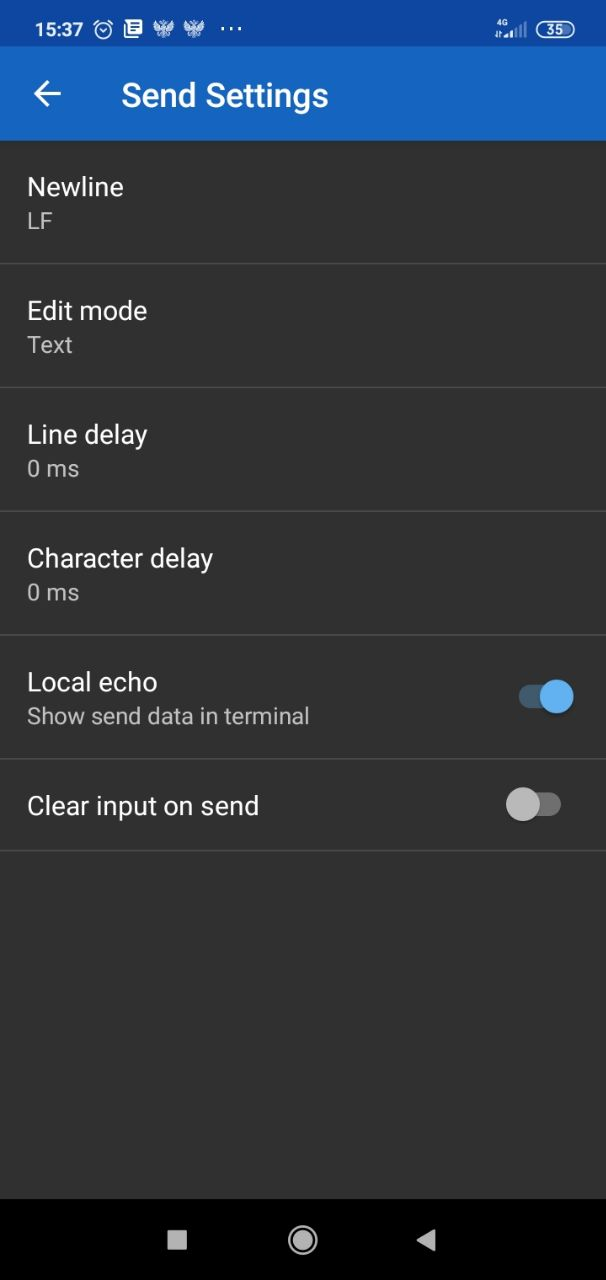
\includegraphics[width=0.32\textwidth]{digifiz_manual/image049.png}
    \caption{Recommended Serial Bluetooth Terminal configuration.}
    \label{fig:sbt-settings}
\end{figure}

Enter commands as space-separated number/value pairs. For example, to store an odometer value of 123\,456~km send \InlineCode{11 123456}. Add 128 to a command number to read its current value (\InlineCode{129 0} reports the speed coefficient). The diagnostic command \InlineCode{adc 0} prints raw sensor readings that help the developers analyse faults.

\section{Configuration parameters}
The primary Bluetooth commands are listed in \autoref{tbl:replica-classic-commands}. Default settings for Generation~1/1.5 and Generation~2 dashboards are summarised in \autoref{tbl:replica-defaults}. Use commands~31--33 only on \ReplicaNextShort{} units; they have no effect on the classic \ReplicaGenOneShort{}.

{\scriptsize
\begin{longtblr}[
    caption = {Classic \ReplicaGenOne{} configuration commands.},
    label = {tbl:replica-classic-commands},
]{
    colspec = {Q[c,0.16\linewidth] Q[l,0.5\linewidth] Q[l]},
    rowsep = 2pt,
}
    \toprule
    \textbf{ID} & \textbf{Name} & \textbf{Description} \\
    \midrule
    22 (or 0) & \InlineCode{PARAMETER\_RPMCOEFFICIENT} & Engine RPM calibration factor. \\
    1 & \InlineCode{PARAMETER\_SPEEDCOEFFICIENT} & Speed calibration factor. \\
    2 & \InlineCode{PARAMETER\_COOLANTTHERMISTORB} & Coolant thermistor beta coefficient. \\
    3 & \InlineCode{PARAMETER\_OILTHERMISTORB} & Oil thermistor beta coefficient. \\
    4 & \InlineCode{PARAMETER\_AIRTHERMISTORB} & Ambient thermistor beta coefficient. \\
    5 & \InlineCode{PARAMETER\_TANKMINRESISTANCE} & Minimum fuel sender resistance (\si{\ohm}). \\
    6 & \InlineCode{PARAMETER\_TANKMAXRESISTANCE} & Maximum fuel sender resistance (\si{\ohm}). \\
    7 & \InlineCode{PARAMETER\_TAU\_COOLANT} & Coolant temperature filter constant. \\
    8 & \InlineCode{PARAMETER\_TAU\_OIL} & Oil temperature filter constant. \\
    9 & \InlineCode{PARAMETER\_TAU\_AIR} & Ambient temperature filter constant. \\
    10 & \InlineCode{PARAMETER\_TAU\_TANK} & Fuel level filter constant. \\
    11 & \InlineCode{PARAMETER\_MILEAGE} & Total odometer value. \\
    12 & \InlineCode{PARAMETER\_DAILY\_MILEAGE} & Trip odometer. \\
    13 & \InlineCode{PARAMETER\_AUTO\_BRIGHTNESS} & Enable automatic brightness adjustment. \\
    14 & \InlineCode{PARAMETER\_BRIGHTNESS\_LEVEL} & Manual brightness level (0--15). \\
    15 & \InlineCode{PARAMETER\_TANK\_CAPACITY} & Fuel tank capacity (litres). \\
    16 & \InlineCode{PARAMETER\_MFA\_STATE} & Active MFA page. \\
    17 & \InlineCode{PARAMETER\_BUZZER\_OFF} & Disable the buzzer (1 disables, 0 enables). \\
    18 & \InlineCode{PARAMETER\_MAX\_RPM} & Tachometer scale (default 8000). \\
    19 & \InlineCode{PARAMETER\_NORMAL\_RESISTANCE\_COOLANT} & Coolant sensor resistance at \SI{25}{\celsius}. \\
    20 & \InlineCode{PARAMETER\_NORMAL\_RESISTANCE\_OIL} & Oil sensor resistance at \SI{25}{\celsius}. \\
    21 & \InlineCode{PARAMETER\_NORMAL\_RESISTANCE\_AMB} & Ambient sensor resistance at \SI{25}{\celsius}. \\
    23 & \InlineCode{PARAMETER\_DOT\_OFF} & Clock colon behaviour (0 blink, 1 solid). \\
    24 & \InlineCode{PARAMETER\_BACKLIGHT\_ON} & Switch on backlight with low beam. \\
    25 & \InlineCode{PARAMETER\_M\_D\_FILTER} & Median filter constant (legacy). \\
    26 & \InlineCode{PARAMETER\_COOLANT\_MAX\_R} & Coolant ``full-scale'' temperature threshold. \\
    27 & \InlineCode{PARAMETER\_COOLANT\_MIN\_R} & Coolant ``1~bar'' temperature threshold. \\
    31--33 & \InlineCode{PARAMETER\_MAINCOLOR\_[RGB]} & Interface colour components (\ReplicaNextShort{} only). \\
    37 & \InlineCode{PARAMETER\_RPM\_FILTER} & RPM filtering aggressiveness. \\
    128 & \InlineCode{PARAMETER\_READ\_ADDITION} & Add to read any parameter. \\
    255 & \InlineCode{PARAMETER\_SET\_HOUR} & Set clock hours (24-hour). \\
    254 & \InlineCode{PARAMETER\_SET\_MINUTE} & Set clock minutes. \\
    253 & \InlineCode{PARAMETER\_RESET\_DAILY\_MILEAGE} & Reset the trip odometer. \\
    252 & \InlineCode{PARAMETER\_RESET\_DIGITAL} & Factory reset and memory initialisation. \\
    \bottomrule
\end{longtblr}}

The Serial Bluetooth Terminal quick buttons are convenient for routine actions such as toggling automatic brightness (\InlineCode{13 0} and \InlineCode{13 1}) or writing colour values. Keep values above \SI{60}{\percent} brightness only for short tests to preserve LED life.

\chapter{Typical situations for setting up the \ReplicaGenOne{}}\label{ch:replica-scenarios}

Before troubleshooting, confirm that the dashboard is the classic \ReplicaGenOne{} (\autoref{ch:replica-setup}). \ReplicaNextLong{} panels use a Wi-Fi portal and are covered in \autoref{ch:replica-next-scenarios}.

\begin{description}
    \item[Bluetooth module not detected] Pair with the dashboard's Bluetooth Classic interface (it normally advertises as \texttt{Digifiz}). Serial Bluetooth Terminal for Android remains the recommended tool: configure the end-of-line character as LF and avoid BLE-only scanners, which cannot discover the module.
    \item[iPhone or iPad cannot connect] \ReplicaGenOneShort{} dashboards use Bluetooth~2.0 and are incompatible with iOS devices. Use an Android phone or a computer running a Bluetooth serial utility.
    \item[Commands ignored on 2024+ firmware] Unlock the command parser by sending \verb|234 123|, then repeat the desired sequence. Store quick-access buttons in Serial Bluetooth Terminal for the values you adjust frequently.
    \item[Speed reading too high or low] Connect through Serial Bluetooth Terminal, drive at an indicated \SI{100}{\kilo\metre\per\hour}, and note the GPS speed. Send \verb|1 <gps_value>| (for example, \verb|1 85|) so \paramname{PARAMETER\_SPEEDCOEFFICIENT} matches the verified GPS speed.
    \item[RPM reading incorrect] Firmware prior to 2024 expects \verb|0 <value>| while current releases use \verb|22 <value>|. Audi engines typically need \verb|22 3000|; halve or double the value (for example, \verb|22 1500| or \verb|22 6000|) until the display matches the tachometer.
    \item[Increase brightness] Disable automatic control with \verb|13 0| and raise the manual level with \verb|14 <value>|. Values between 45 and 55 brighten the display substantially; avoid levels above 60 to preserve LED life. Re-enable the photodiode later with \verb|13 1|.
    \item[Setting the clock] Use Serial Bluetooth Terminal to send \verb|255 <hours>| followed by \verb|254 <minutes>|. Examples: \verb|255 23|, \verb|254 55| sets 23:55; \verb|255 14|, \verb|254 30| sets 14:30; \verb|255 2|, \verb|254 28| sets 02:28.
    \item[Fuel gauge issues] Disconnect the vehicle battery before probing.\begin{itemize}
        \item If the display drifts from 60 to 0, measure the sender resistance between the harness pin and ground; valid readings are typically \SIrange{30}{300}{\ohm}. Clean the connector and confirm the signal reaches the main board.
        \item If the gauge is pegged full, look for a short to ground below \SI{5}{\ohm} on the sender line and repair it.
        \item If the reading never changes, compare the sender resistance with full and empty tanks. Replace the sensor if it stays constant.
    \end{itemize}
    \item[Fuel flow values seem wrong] The flow channel is emulated unless an intake-manifold pressure sensor is fitted. Treat the reading as indicative rather than absolute.
    \item[Coolant gauge inaccurate] Adjust \paramname{PARAMETER\_COOLANT\_MIN\_R} and \paramname{PARAMETER\_COOLANT\_MAX\_R}. Example: \verb|27 30| shortens the scale so that the ``1~bar'' mark aligns with roughly \SI{30}{\celsius}.
    \item[Oil or ambient temperature readings missing] A reading of \texttt{-999} or a stuck value indicates a sensor issue. With the battery disconnected and the engine cold, measure the sensor resistance between the harness pin and ground. Oil sensors should read about \SI{2}{\kilo\ohm} \ensuremath{\pm}\SI{0.3}{\kilo\ohm}; ambient sensors about \SI{10}{\kilo\ohm} \ensuremath{\pm}\SI{2}{\kilo\ohm}. Adjust \paramname{PARAMETER\_NORMAL\_RESISTANCE\_OIL} (command~20) or \paramname{PARAMETER\_NORMAL\_RESISTANCE\_AMB} (command~21) if the display needs fine-tuning. Persistent faults should be documented with \verb|adc 0| logs and escalated to PHOL-LABS Kft support.
\end{description}

Collect raw sensor data with \verb|adc 0| if the problem persists and share the results with the dashboard developers for analysis.

\chapter{Marking and sealing}\label{ch:marking}

\begin{itemize}
    \item Each dashboard may be marked with the model number corresponding to its instrument-cluster variant.
    \item Export batches can include additional markings applied by the importing organisation.
    \item The \ReplicaGenOne{} is not sealed; no tamper seals are fitted at the factory.
\end{itemize}

\chapter{Package}\label{ch:package}

\begin{enumerate}
    \item For transport, wrap the instrument panel set in bubble wrap and place it in a rigid cardboard box.
    \item Alternative packaging is acceptable provided it protects the dashboard during transport and storage.
\end{enumerate}

\chapter{Storage and transportation rules}\label{ch:storage}

\begin{itemize}
    \item Transportation conditions must comply with the general freight rules applicable to each transport mode (GOST~23216-78).
    \item Packaged dashboards may be shipped by road, rail, river, or air transport.
    \item Store the instrument panel inside the vehicle cabin or in a heated room between \SI{15}{\celsius} and \SI{40}{\celsius}. Protect the unit from direct sunlight, although storage behind vehicle glass is permissible.
\end{itemize}


\appendix
\chapter{Reference Tables} \label{appendix:reference}

\section{Classic \ReplicaGenOne{} Command Reference}

The classic Replica firmware shares most commands with \ReplicaNextShort{}.
Commands 31--33 (colour control) are only active on \ReplicaNextShort{} units; other commands apply equally to both generations.

\begin{table}[htbp]
    \centering
    \caption{Primary configuration commands for classic \ReplicaGenOne{} dashboards.}
    \label{tbl:replica-commands}
    {\scriptsize
    \begin{tblr}{
        colspec = {Q[c,0.16\linewidth] Q[l,0.5\linewidth] Q[l]},
        rowsep = 2pt,
    }
        \toprule
        \textbf{Command} & \textbf{Name} & \textbf{Description} \\
        \midrule
        22 (or 0) & \InlineCode{PARAMETER\_RPMCOEFFICIENT} & Engine RPM calibration factor. \\
        1  & \InlineCode{PARAMETER\_SPEEDCOEFFICIENT} & Speed calibration factor. \\
        2  & \InlineCode{PARAMETER\_COOLANTTHERMISTORB} & Coolant thermistor beta coefficient. \\
        3  & \InlineCode{PARAMETER\_OILTHERMISTORB} & Oil thermistor beta coefficient. \\
        4  & \InlineCode{PARAMETER\_AIRTHERMISTORB} & Ambient thermistor beta coefficient. \\
        5  & \InlineCode{PARAMETER\_TANKMINRESISTANCE} & Minimum fuel sender resistance. \\
        6  & \InlineCode{PARAMETER\_TANKMAXRESISTANCE} & Maximum fuel sender resistance. \\
        7--10 & \InlineCode{PARAMETER\_TAU\_\textit{X}} & Filtering constants for coolant, oil, air, and fuel level.
        \\
        11 & \InlineCode{PARAMETER\_MILEAGE} & Total odometer value. \\
        12 & \InlineCode{PARAMETER\_DAILY\_MILEAGE} & Trip odometer. \\
        13 & \InlineCode{PARAMETER\_AUTO\_BRIGHTNESS} & Automatic brightness enable. \\
        14 & \InlineCode{PARAMETER\_BRIGHTNESS\_LEVEL} & Manual brightness level. \\
        15 & \InlineCode{PARAMETER\_TANK\_CAPACITY} & Fuel tank capacity. \\
        16 & \InlineCode{PARAMETER\_MFA\_STATE} & Active MFA mode. \\
        17 & \InlineCode{PARAMETER\_BUZZER\_OFF} & Disable buzzer (Replica only). \\
        18 & \InlineCode{PARAMETER\_MAX\_RPM} & Tachometer scaling (7000 default). \\
        19--21 & \InlineCode{PARAMETER\_NORMAL\_RESISTANCE\_\textit{X}} & Sensor resistances at \SI{25}{\celsius} for coolant, oil, and ambient inputs. \\
        23 & \InlineCode{PARAMETER\_DOT\_OFF} & Clock colon behaviour. \\
        24 & \InlineCode{PARAMETER\_BACKLIGHT\_ON} & Enable backlight when low beam is active. \\
        25 & \InlineCode{PARAMETER\_M\_D\_FILTER} & Median filter constant. \\
        26 & \InlineCode{PARAMETER\_COOLANT\_MAX\_R} & Coolant sensor threshold for full-scale indication. \\
        27 & \InlineCode{PARAMETER\_COOLANT\_MIN\_R} & Coolant sensor threshold for ``1~bar'' indication. \\
        31--33 & \InlineCode{PARAMETER\_MAINCOLOR\_[RGB]} & UI colour components (\ReplicaNextShort{} only). \\
        37 & \InlineCode{PARAMETER\_RPM\_FILTER} & RPM filtering aggressiveness. \\
        128 & \InlineCode{PARAMETER\_READ\_ADDITION} & Add 128 to read the current value of a command. \\
        255 & \InlineCode{PARAMETER\_SET\_HOUR} & Set clock hours. \\
        254 & \InlineCode{PARAMETER\_SET\_MINUTE} & Set clock minutes. \\
        253 & \InlineCode{PARAMETER\_RESET\_DAILY\_MILEAGE} & Reset trip odometer. \\
        252 & \InlineCode{PARAMETER\_RESET\_DIGITAL} & Factory reset of stored parameters. \\
        \bottomrule
    \end{tblr}}
\end{table}

\section{Classic \ReplicaGenOneShort{} Default Values}

\begin{table}[htbp]
    \centering
    \caption{Default configuration for the classic \ReplicaGenOne{}.}
    \label{tbl:replica-defaults}
    {\scriptsize
    \begin{tblr}{
        colspec = {Q[l,0.55\linewidth] Q[c,0.16\linewidth] Q[l]},
        rowsep = 2pt,
    }
        \toprule
        \textbf{Parameter} & \textbf{Default} & \textbf{Notes} \\
        \midrule
        \InlineCode{PARAMETER\_RPMCOEFFICIENT} & 3000 &  \\
        \InlineCode{PARAMETER\_SPEEDCOEFFICIENT} & 100 &  \\
        \InlineCode{PARAMETER\_COOLANTTHERMISTORB} & 4000 &  \\
        \InlineCode{PARAMETER\_OILTHERMISTORB} & 4000 &  \\
        \InlineCode{PARAMETER\_AIRTHERMISTORB} & 3812 & 3600 on Gen~2. \\
        \InlineCode{PARAMETER\_TANKMINRESISTANCE} & 35 & Ohms. \\
        \InlineCode{PARAMETER\_TANKMAXRESISTANCE} & 265 & Ohms. \\
        \InlineCode{PARAMETER\_TAU\_COOLANT} & 2 &  \\
        \InlineCode{PARAMETER\_TAU\_OIL} & 2 &  \\
        \InlineCode{PARAMETER\_TAU\_AIR} & 2 &  \\
        \InlineCode{PARAMETER\_TAU\_TANK} & 2 &  \\
        \InlineCode{PARAMETER\_MILEAGE} & Vehicle-specific & Preserve existing odometer. \\
        \InlineCode{PARAMETER\_DAILY\_MILEAGE} & 0 &  \\
        \InlineCode{PARAMETER\_AUTO\_BRIGHTNESS} & 1 & Enabled. \\
        \InlineCode{PARAMETER\_BRIGHTNESS\_LEVEL} & 7 or 13 & Typical values for Gen~1/1.5. \\
        \InlineCode{PARAMETER\_TANK\_CAPACITY} & 63 & Litres. \\
        \InlineCode{PARAMETER\_MFA\_STATE} & 0 &  \\
        \InlineCode{PARAMETER\_BUZZER\_OFF} & 1 & Buzzer disabled. \\
        \InlineCode{PARAMETER\_MAX\_RPM} & 8000 & 7000 on earlier clusters. \\
        \InlineCode{PARAMETER\_NORMAL\_RESISTANCE\_COOLANT} & 1000 & \si{\ohm} at \SI{25}{\celsius}. \\
        \InlineCode{PARAMETER\_NORMAL\_RESISTANCE\_OIL} & 1000 & \si{\ohm} at \SI{25}{\celsius}. \\
        \InlineCode{PARAMETER\_NORMAL\_RESISTANCE\_AMB} & 2991 & \si{\ohm} at \SI{25}{\celsius}. \\
        \InlineCode{PARAMETER\_DOT\_OFF} & 0 & Blinking colon. \\
        \InlineCode{PARAMETER\_BACKLIGHT\_ON} & 1 & Enabled. \\
        \InlineCode{PARAMETER\_M\_D\_FILTER} & 65535 &  \\
        \InlineCode{PARAMETER\_COOLANT\_MAX\_R} & 120 & \si{\celsius}. \\
        \InlineCode{PARAMETER\_COOLANT\_MIN\_R} & 60 & \si{\celsius}. \\
        \InlineCode{PARAMETER\_MAINCOLOR\_[RGB]} & -- & Colour commands not active on classic Replica. \\
        \InlineCode{PARAMETER\_RPM\_FILTER} & 70 &  \\
        \InlineCode{PARAMETER\_UPTIME} & 0 &  \\
        \bottomrule
    \end{tblr}}
\end{table}

\section{Change Log} \label{app:change-log}

\begin{table}[htbp]
    \centering
    \caption{Document change registration sheet.}
    \label{tbl:change-log}
    {\scriptsize
    \begin{tblr}{
        colspec = {Q[c,0.12\linewidth] Q[l] Q[c,0.18\linewidth] Q[c,0.2\linewidth] Q[c,0.16\linewidth] Q[c,0.18\linewidth]},
        rowsep = 2pt,
    }
        \toprule
        \textbf{Change} & \textbf{Affected sheets} & \textbf{Document No.} & \textbf{Incoming reference} & \textbf{Signature} & \textbf{Date} \\
        \midrule
        1 & 04.10.2022 & -- & -- & -- & 04~Oct~2022 \\
        2 & 31.08.2023 & -- & -- & -- & 31~Aug~2023 \\
        3 & 05.08.2024 & -- & -- & -- & 05~Aug~2024 \\
        \bottomrule
    \end{tblr}}
\end{table}


\backmatter
\references

\end{document}
